%% =====================================================================
%% Ramis basin manuscript (REVISED VERSION WITH CITATIONS)
%% Elsevier CAS single-column class (cas-sc.cls).
%%
%% REVISION NOTES:
%%  - Introduction, Methods, Discussion rewritten with targeted citations
%%    from the provided bibliography annotations.
%%  - Citation style: \citep{} for parenthetical, \citet{} for narrative.
%% =====================================================================
\documentclass[a4paper,fleqn]{cas-sc}

\usepackage[authoryear,longnamesfirst]{natbib}
\usepackage{amsmath,amssymb}
\usepackage{booktabs}
\usepackage{graphicx}
\usepackage{tabularx}
\usepackage{threeparttable}
\usepackage{multirow}
\usepackage{siunitx}
\usepackage{xspace}
\usepackage{url}
\usepackage{float}
\usepackage{enumitem}

% Editorial macros for units and breakable audit identifiers
\newcommand{\cms}{m$^3$\,s$^{-1}$}
\newcommand{\modelid}[1]{\begingroup\urlstyle{same}\path{#1}\endgroup}
\newcommand{\backendid}[1]{\begingroup\urlstyle{same}\path{#1}\endgroup}


\begin{document}
\let\WriteBookmarks\relax
\def\floatpagepagefraction{1}
\def\textpagefraction{.001}

\shorttitle{Stochastic physical-ensemble quantiles for streamflow hybridization}
\shortauthors{Zevallos}

\title[mode = title]{Stochastic Physical-Ensemble Quantiles Improve Hybrid Daily Streamflow Simulation in the High-Andean Ramis Basin}

% First author
\author[1]{Jose Zevallos}[orcid=0000-0002-6023-8665]
\cormark[1]
\ead{20240318@lamolina.edu.pe}
\credit{Conceptualization of this study, Methodology, Formal analysis, Writing -- original draft}

% Address/affiliation
\affiliation[1]{organization={Centro de Investigaci\'{o}n y Tecnolog\'{i}a del Agua (CITA), Universidad de Ingenier\'{i}a y Tecnolog\'{i}a (UTEC)},
                addressline={Jr. Medrano Silva 165, Barranco},
                city={Lima},
                postcode={15063},
                state={Lima},
                country={Peru}}

\cortext[1]{Corresponding author.}

%% =====================================================================
%% ABSTRACT
%% =====================================================================
\begin{abstract}
Hybrid hydrological modelling combines process-based structure with ML,
but often leaves unclear which component drives improved streamflow
prediction. We evaluate a controlled stochastic physical--ML framework
for daily streamflow simulation in the high-Andean Ramis basin, Lake
Titicaca system, Peru. The framework couples a RAMIS rainfall--runoff
core, an optional baseflow reservoir, L\'{e}vy-type stochastic
perturbations, Monte Carlo ensembles, and ML emulators trained from
observed forcings or ensemble descriptors. Nine experiments (E0--E8)
were evaluated over a common validation window (8 January 2009 to
31 December 2020; $n=4367$ days), with leakage and backend audits in
the evidence chain.

Quantile descriptors from the stochastic ensemble provided the largest
robust gain. The gradient-boosting quantile hybrid reached NSE\,=\,0.740
and KGE\,=\,0.810, improving NSE by 0.311 over the stochastic physical
baseline and by 0.165 over the pure ML baseline. Replacing ensemble-mean
with ensemble-quantile features alone added 0.114 NSE, confirming that
distributional physical descriptors carry information beyond a single
mean trajectory. The baseflow reservoir modestly improved the
deterministic baseline; direct L\'{e}vy perturbations produced
inconsistent point-prediction gains. Stochastic bands were strongly
underdispersive (PICP\,=\,0.004 vs nominal 0.95), making the ensemble
more useful as ML features than as calibrated uncertainty. The best
numerical run (NSE\,=\,0.849) was labelled GRU but executed as a
fallback perceptron; it is not evidence of recurrent-network
superiority. These findings support stochastic physical--ML
hybridization while showing that uncertainty calibration, low-flow
correction and backend-aware reporting remain essential.
\end{abstract}

\begin{highlights}
\item Ensemble quantiles provided the largest backend-consistent hybrid gain.
\item The quantile hybrid improved NSE by 0.311 over stochastic RAMIS.
\item L\'{e}vy perturbations informed ML features but underdispersed intervals.
\item Backend and leakage audits constrained claims for GRU-labelled runs.
\item The ablation separated memory, stochasticity, ML and descriptors.
\end{highlights}

\begin{keywords}
Daily streamflow simulation \sep Stochastic hydrological modelling \sep
Physical--ML hybridization \sep Ensemble quantiles \sep
Uncertainty diagnostics \sep High-Andean basin
\end{keywords}

\maketitle

%% =====================================================================
%% 1. INTRODUCTION
%% =====================================================================
\section{Introduction}\label{sec:introduction}

Reliable daily streamflow simulation remains a central problem in
surface-water hydrology, particularly in basins where observations are
sparse, hydroclimatic variability is strong and operational decisions
must still be supported by defensible discharge estimates
\citep{razavi2013streamflow,guo2021regionalization}. These conditions
are characteristic of many high-elevation Andean catchments. In the
Peruvian Altiplano, precipitation is strongly seasonal, monitoring
networks are sparse relative to the spatial heterogeneity of rainfall,
and discharge dynamics are shaped by the alternation between sharp
wet-season runoff response and sustained dry-season low flows
\citep{condom2004transient,zubieta2018hydrological,lima2025modeling}.
Such settings expose a persistent limitation of classical
rainfall--runoff modelling: even when a conceptual model captures the
main water-balance controls, simplified storage structures, uncertain
parameters and imperfect meteorological inputs can lead to structural
errors that become particularly visible under low-flow, flashy or
climatically contrasting conditions
\citep{van2013influence,nauditt2017conceptual,ragettli2014evaluation}.

Machine-learning (ML) models offer a complementary route because they
can learn nonlinear rainfall--runoff relations directly from data. Large
sample studies have shown that recurrent and other data-driven models
can match or outperform lumped conceptual models in daily streamflow
prediction, including in regional and basin-scale benchmarks
\citep{kratzert2019towards,lees2021benchmarking,arsenault2022continuous}.
However, predictive skill alone does not eliminate hydrological risk.
Purely data-driven models may be sensitive to distributional shifts,
training-period representativeness, extrapolation to extremes and the
absence of explicit physical constraints
\citep{frame2021deep,zhong2023developing}. In data-scarce basins, their
performance also depends strongly on whether antecedent hydrological
state information is available, because rainfall inputs alone may be
insufficient to represent catchment memory
\citep{adnan2021comparison,okkan2021embedding}. The practical question
is therefore not whether process-based or ML models are universally
superior, but how physical structure and empirical flexibility can be
combined without obscuring the source of any improvement.

Hybrid physical--ML modelling addresses this question by using process
simulations, physically derived states or synthetic physically
consistent samples as inputs to an empirical emulator. This strategy has
improved runoff simulation in several configurations, including
conceptual-model correction, nested hybrid rainfall--runoff modelling,
physics-guided deep learning and process-driven deep learning
\citep{mekonnen2015hybrid,mohammadi2022ihacres,okkan2021embedding,yang2020physical,xie2021physics,li2024process,zhu2025hybrid}.
Most of these studies, however, pass forward a deterministic physical
trajectory. That design preserves part of the process information but
collapses the conditional distribution of the simulated response into a
single value. For stochastic rainfall--runoff transformation, this is a
strong simplification: uncertainty in precipitation, model structure and
hydrological memory propagates nonlinearly into discharge and can alter
both peak timing and magnitude
\citep{gabellani2007propagation,hong2006uncertainty}. It also limits the
ability of the hybrid model to exploit distributional descriptors such
as ensemble quantiles, which are closely related to hydrological
signatures and to probabilistic forecasting diagnostics
\citep{guo2021regionalization,papacharalampous2022review}.

A recent stochastic hybridization study by
\citet{houenafa2025hybridization} showed that mean and quantile
descriptors of a L\'{e}vy-driven stochastic discharge ensemble
can improve ML-based rainfall--runoff prediction. This result is
important because it moves physical--ML hybridization from deterministic
state correction toward distribution-aware physical descriptors. Yet it
also leaves three issues unresolved. First, the gain from the hybrid
pipeline may come from several components---hydrological memory,
stochastic perturbations, the ML correction itself or the use of
quantile rather than mean ensemble descriptors---and these effects are
not identifiable from a single best-model comparison. Second, a
stochastic ensemble that improves point prediction is not necessarily a
calibrated predictive interval; coverage, sharpness and interval scores
must be evaluated separately. Third, reproducibility claims require that
reported model labels match the backend that actually produced the
results, especially when reported model labels differ from the model actually
used to generate predictions.

This study addresses these gaps using a controlled stochastic
physical--ML ablation design for daily streamflow simulation in the
high-Andean Ramis basin, the principal tributary of Lake Titicaca. The
modelling chain couples a lumped RAMIS rainfall--runoff core, an
optional linear baseflow reservoir, L'{e}vy-type stochastic
perturbations, Monte Carlo physical ensembles and ML emulators trained
either from observed forcings or from physical-ensemble descriptors. The
purpose is to decompose which modelling components are responsible for
performance gains. Nine controlled experiments (E0--E8;
Table~\ref{tab:experiment-matrix}) are therefore evaluated over a
common validation window using a common modelling and evaluation design
(Fig.~\ref{fig:method-workflow}). The ablation design isolates the
incremental roles of baseflow memory, stochastic forcing, ML correction
and descriptor choice.

The manuscript makes four specific contributions. First, it transfers
stochastic physical--ML quantile hybridization to a high-Andean,
strongly seasonal and data-scarce Altiplano basin, providing a contrast
to previous applications outside this hydroclimatic setting. Second, it
shows whether ensemble mean or ensemble quantiles carry the more useful
physical information for ML correction. Third, it evaluates the same
stochastic ensemble both as a source of predictive features and as a
candidate uncertainty band through PICP, PINAW and Winkler diagnostics.
Fourth, it embeds temporal-leakage and backend audits into the evidence
chain, following the broader call for transparent and reproducible
hydrological modelling \citep{hall2021hydrologist}. A key audit finding
is stated explicitly: the experiments labelled as GRU in the current
run were executed with a fallback multilayer perceptron on flattened
sequences, not with a true recurrent backend. They are therefore
interpreted as GRU-labelled sequential hybrids under fallback execution,
not as evidence of recurrent-network superiority
\citep{kratzert2018rainfall}.

%% =====================================================================
%% 2. MATERIALS AND METHODS
%% =====================================================================
\section{Materials and methods}\label{sec:methods}


\subsection{Study area}\label{subsec:study-area}

The Ramis River basin is located in the high-Andean Altiplano of
southern Peru and drains towards Lake Titicaca. The basin is therefore
part of a closed lacustrine system in which river inflow, precipitation
and evaporation exert strong control on lake-level variability
\citep{cross2001late,condom2004transient,lima2025modeling}. Previous
regional studies show that the hydrology of the Titicaca system is
controlled mainly by rainfall and evapotranspiration variability,
whereas snowmelt, ice melt and net irrigation withdrawals have a
secondary role at the lake-basin scale \citep{lima2025modeling}. This
regional behaviour makes the Ramis basin a relevant test case for a
rainfall--runoff modelling design that combines process-based memory,
stochastic forcing and machine-learning correction.

The basin is characterized by high elevation, sparse hydroclimatic
monitoring and a strongly seasonal precipitation regime. Rainfall is
concentrated during the austral summer wet season, while the dry season
is associated with prolonged recession and low-flow persistence
\citep{condom2004transient,nauditt2017conceptual,lima2025modeling}.
Such hydroclimatic asymmetry is challenging for lumped conceptual
models because a single storage response may be unable to represent both
wet-season peaks and dry-season baseflow. It is also challenging for
purely data-driven models, which may learn strong seasonal correlations
without representing the storage mechanisms that maintain discharge
between rainfall events \citep{van2013influence,lees2021benchmarking}.
Daily discharge observations used in this study correspond to the
Puente Ramis gauging station operated by SENAMHI-Peru.

Figure~\ref{fig:study-area} provides the geographical frame of the
analysis. The delineated catchment, drainage network and model outlet
identify the spatial support over which gridded meteorological products
were aggregated before being used in the lumped rainfall--runoff model.
This step is essential because the model is evaluated at daily time step
and catchment scale; therefore, the consistency between the outlet,
catchment boundary, drainage network and meteorological forcing domain
directly defines the hydrological unit being simulated.

\begin{figure*}[t]
\centering
\IfFileExists{figures/study_area_ramis.png}{%
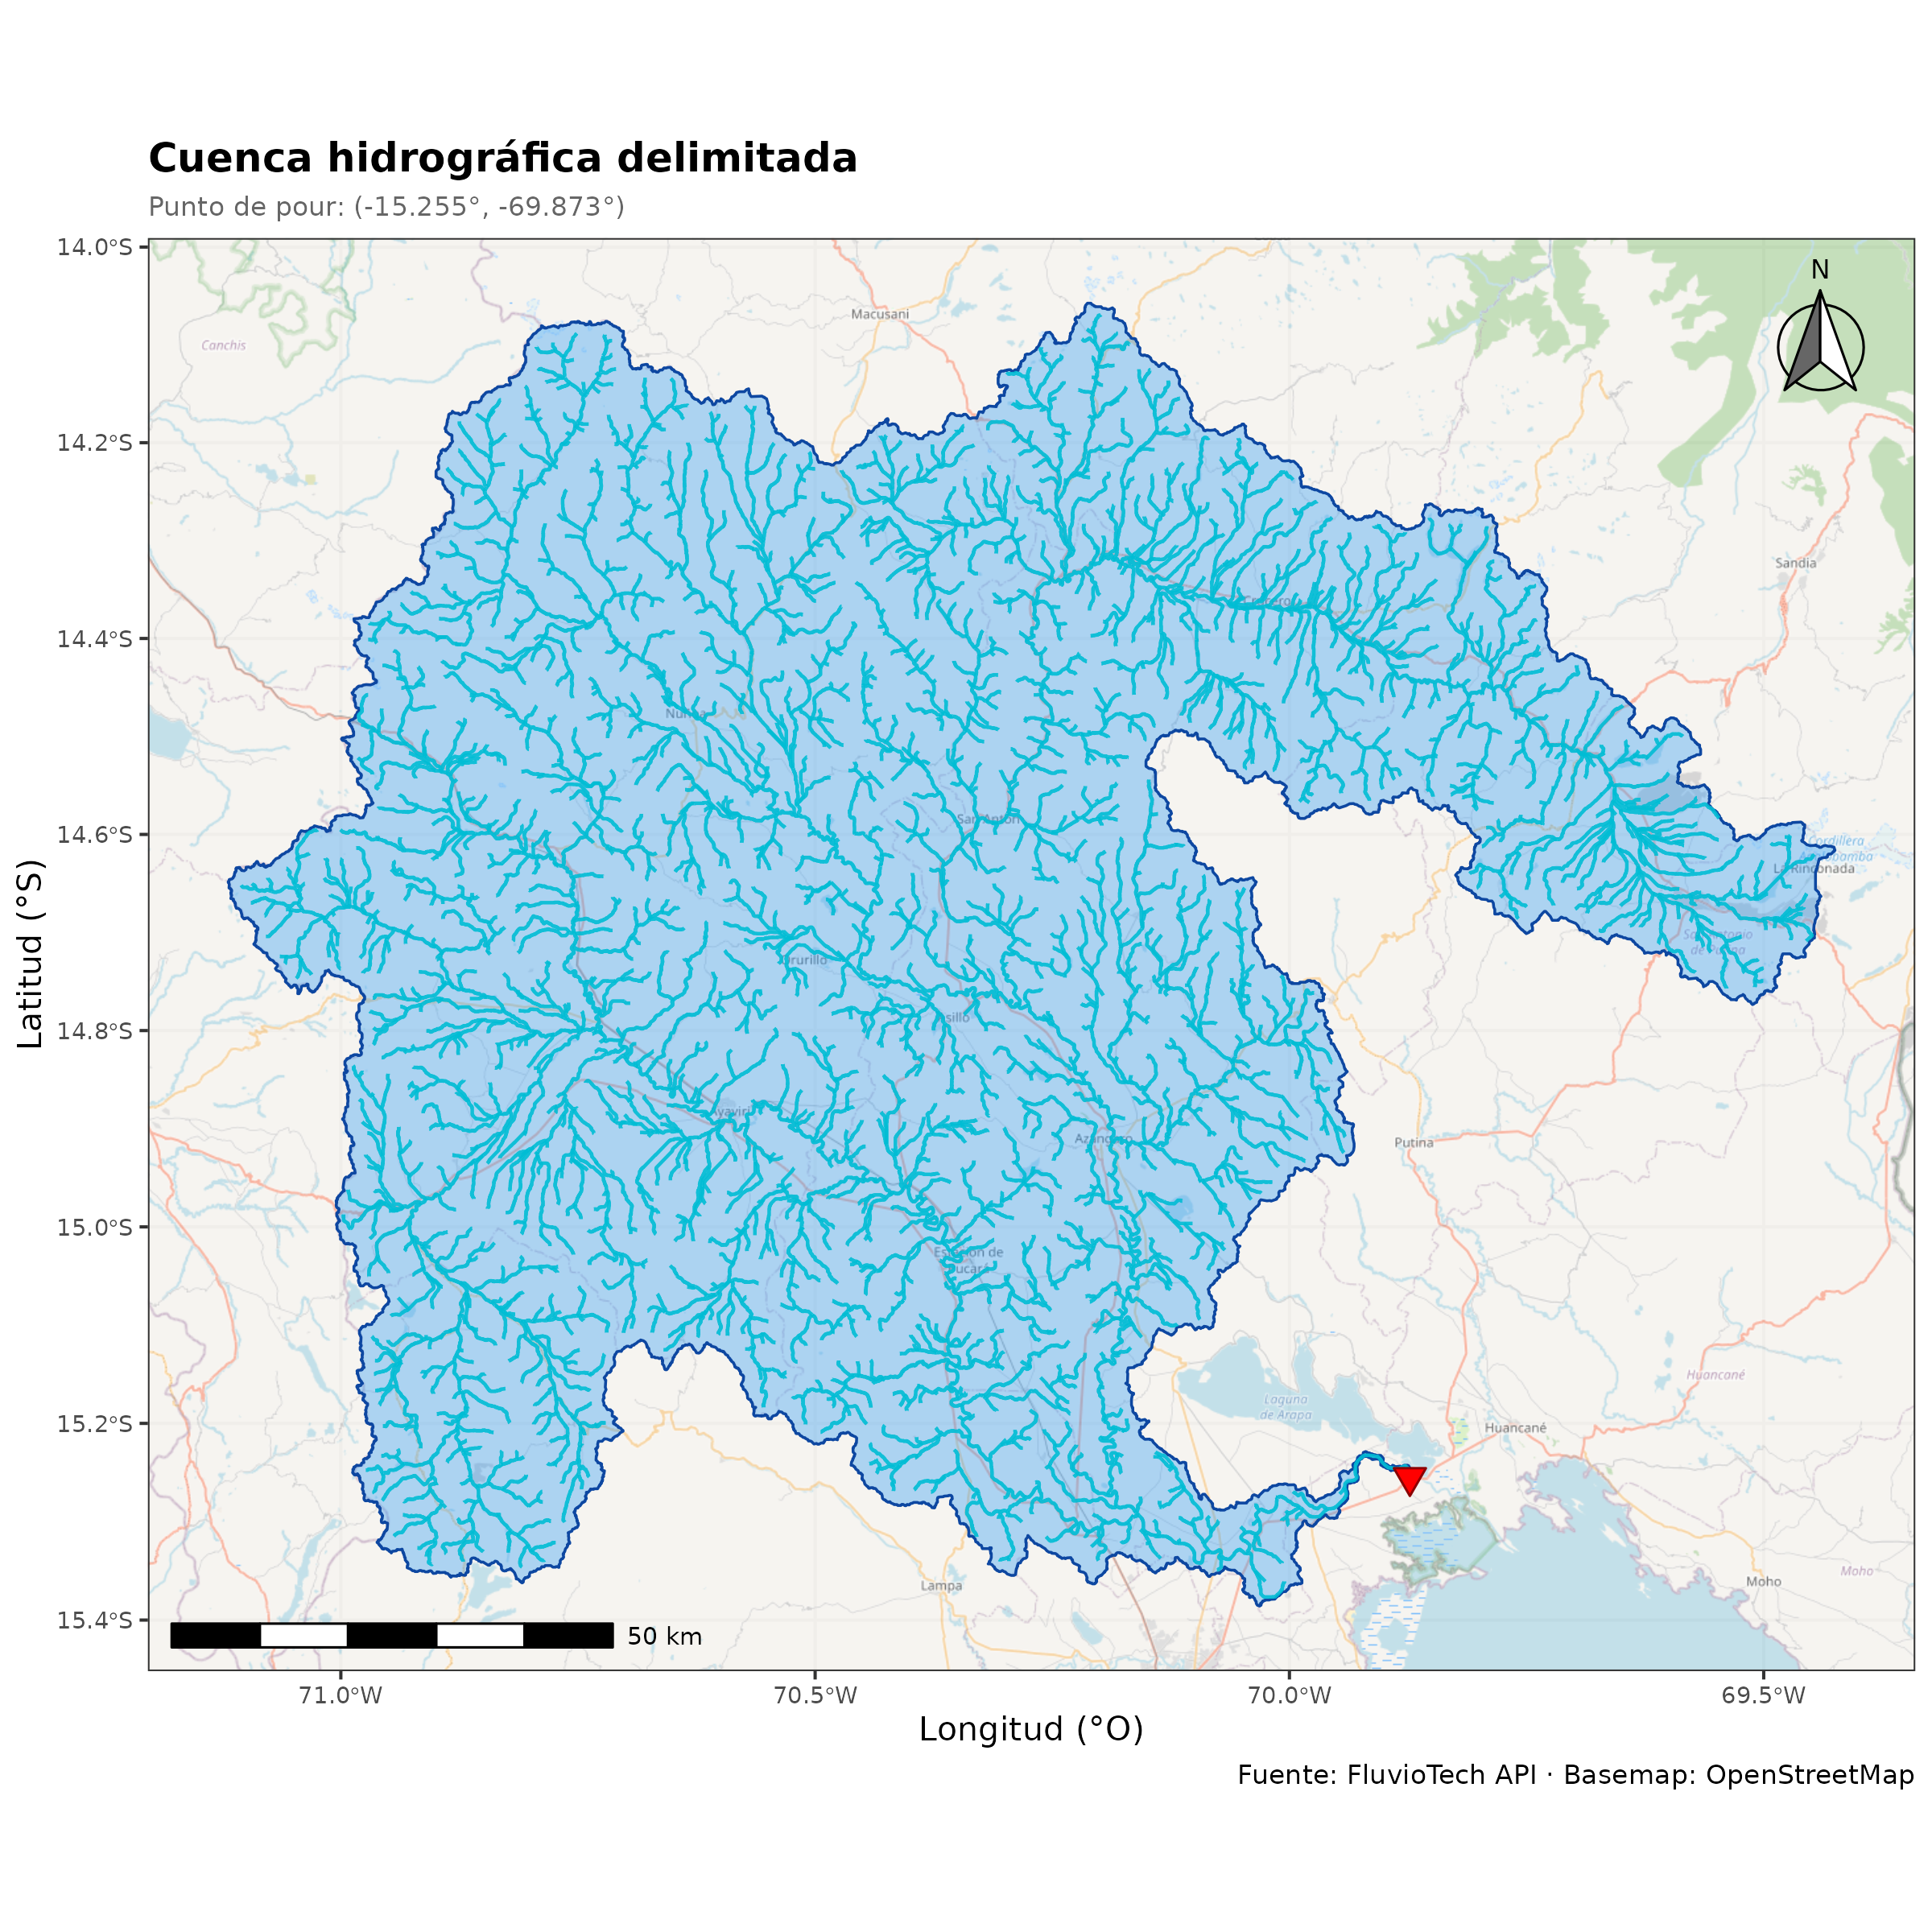
\includegraphics[width=0.92\textwidth]{figures/study_area_ramis.png}%
}{%
\fbox{\parbox[c][0.32\textheight][c]{0.90\textwidth}{\centering
Placeholder for the final study-area map. Replace this box with
\texttt{figures/study\_area\_ramis.png} before submission.}}%
}
\caption{Geographical setting of the Ramis River basin in the
high-Andean Altiplano of southern Peru. The delineated catchment drains
towards Lake Titicaca; the drainage network indicates the main flow
paths represented at catchment scale, and the red marker denotes the
model outlet or pour point used for basin delineation
(15.2550$^{\circ}$S, 69.8730$^{\circ}$W). The map defines the spatial
support used to aggregate gridded precipitation from PISCOp v3.0 and
minimum and maximum air temperature from PISCOt v1.2 into daily
catchment-scale forcings for the lumped rainfall--runoff experiments.}
\label{fig:study-area}
\end{figure*}

%% [AUTHOR ACTION BEFORE SUBMISSION]
%% Insert the official gauged drainage area, station coordinates, gauge
%% elevation and complete record period from SENAMHI/ANA metadata. These
%% details were not included in the materials available for this phase
%% and should not be inferred.

\subsection{Hydro-meteorological data and temporal protocol}
\label{subsec:data-protocol}

The modelling unit is a daily catchment-scale hydro-meteorological
record composed of precipitation ($P_t$), minimum and maximum air
temperature ($T_{\min,t}$ and $T_{\max,t}$), potential
or reference evapotranspiration ($PET_t$) and observed streamflow
($Q^{obs}_t$). Daily precipitation was obtained from the PISCOp v3.0
gridded rainfall product. PISCOp v3.0 is used here as the updated 2026
release of the PISCO precipitation product family; the published
construction of the PISCOp v2.1 rainfall dataset is documented by
\citet{aybar2020construction}. This citation is used to document the
PISCO rainfall dataset family and its gridded-data construction
principles, whereas the specific precipitation input used in this study
corresponds to version~3.0.

Daily minimum and maximum air temperature were obtained from PISCOt
v1.2, a high-resolution gridded daily temperature product for Peru
\citep{huerta2023high}. Precipitation and temperature grids were
spatially aggregated over the delineated Ramis catchment
(Fig.~\ref{fig:study-area}) to obtain basin-mean daily forcing series
for the lumped model. Observed streamflow was taken from the Puente
Ramis gauging station operated by SENAMHI-Peru. All forcing and
discharge series were then aligned at daily time step before model
calibration, ML training and validation.

Potential evapotranspiration was estimated from the PISCOt v1.2
minimum and maximum temperature series using the Hargreaves--Samani
temperature-based formulation \citep{hargreaves1985reference}:
\begin{equation}
PET_t = 0.0023\,R_{a,t}\,(T_{mean,t}+17.8)
        \sqrt{\max(T_{\max,t}-T_{\min,t},0)},
\label{eq:hargreaves-samani}
\end{equation}
where $T_{mean,t}=(T_{\max,t}+T_{\min,t})/2$ and $R_{a,t}$ is
extraterrestrial radiation expressed as equivalent evaporation depth.
With this convention, $PET_t$ is expressed in mm~d$^{-1}$. The
non-negative thermal-amplitude term avoids numerical artefacts if the
processed gridded temperature series contain equal or nearly equal
minimum and maximum values.

The rainfall--runoff core uses an effective precipitation input defined
as
\begin{equation}
P^{eff}_t = \max(P_t - PET_t,\;0),
\label{eq:peff}
\end{equation}
which provides a non-negative approximation of the water available for
runoff generation after atmospheric demand has been accounted for.

All experiments follow the same chronological split. Model calibration
and ML training use data from 8~September~1991 to 31~December~2008,
whereas validation uses data from 8~January~2009 to 31~December~2020.
The final comparative assessment is computed over the common validation
intersection of all experiments, comprising $n=4367$ daily samples. This
common-window design prevents unequal evaluation support across
physical, ML and hybrid configurations and is especially important for
experiments that require lagged predictors or sequence construction.

Temporal leakage was controlled at four levels. First, lagged predictors
were constructed only from present or past information. Second,
sequence samples were generated independently within the training and
validation partitions. Third, scalers and transformations used by ML
models were fitted exclusively on training data and then applied to
validation data. Fourth, flow-regime thresholds used for diagnostic
stratification were estimated from training observations only. These
controls follow the broader hydrological ML recommendation that model
selection and preprocessing must preserve temporal ordering
\citep{arsenault2022continuous,chen2013finding}. The corresponding
audit status is reported in Table~\ref{tab:reproducibility}.

\subsection{Lumped rainfall--runoff core}\label{subsec:physical-core}

The physical component evaluated here is a lumped stochastic
rainfall--runoff model, not a spatially distributed hydraulic or
hydrodynamic solver. The process-based component is therefore described
as a catchment-scale discharge-dynamics model. Its fast-flow state is
represented by the recurrence
\begin{equation}
x_t = \left(1 - \frac{\mu}{\lambda}\right)x_{t-1} + P^{eff}_t,
\label{eq:ramis-state}
\end{equation}
where $\mu>0$ and $\lambda>0$ regulate catchment memory and recession
stability. The parameter constraint $0<\mu/\lambda<1$ ensures a stable,
non-oscillatory memory factor.

The fast-flow discharge component is updated as
\begin{equation}
Q^{fast}_t = Q^{fast}_{t-1}
  - \frac{\mu}{\lambda}\,Q_0
    \left(\frac{\max(Q^{fast}_{t-1},0)}{Q_0}\right)^{2\mu-1}
  + \frac{\alpha_A}{\lambda}\,x_{t-1}
  + \sigma\,Q^{fast}_{t-1}\,\Delta L_t,
\label{eq:ramis-fast}
\end{equation}
where $Q_0$ is a reference discharge, $\alpha_A$ is an empirical
conversion factor, $\sigma$ controls stochastic amplitude and
$\Delta L_t$ is a stochastic increment. In deterministic experiments,
the stochastic term is inactive. Negative simulated discharge is clipped
to zero when non-negative physical post-processing is enabled.

The recurrence in Eqs.~\ref{eq:ramis-state}--\ref{eq:ramis-fast}
represents catchment-scale nonlinearity through aggregated storage
behaviour. This interpretation is consistent with recession analyses in
which nonlinear catchment response can emerge from heterogeneous linear
storage elements rather than from a single local nonlinear mechanism
\citep{harman2009power}. In this setting, the parameter $\mu$ acts as a
shape parameter controlling the effective recession behaviour of the
lumped storage system.

\subsection{Linear baseflow reservoir}\label{subsec:baseflow}

An optional linear reservoir is used to represent hydrological memory
beyond the fast-flow recurrence. This addition is motivated by previous
work in the Titicaca region showing that groundwater storage fluxes are
important for explaining seasonal runoff persistence and dry-season
baseflow \citep{nauditt2017conceptual}. The reservoir also provides a
controlled way to test whether adding a simple memory component improves
simulation skill before introducing stochastic perturbations or ML
correction.

Recharge to the baseflow store is proportional to effective
precipitation:
\begin{equation}
R_t = c_r\,\alpha_A\,P^{eff}_t,
\label{eq:recharge}
\end{equation}
where $c_r\in[0,1]$ is the recharge coefficient. Storage and baseflow
discharge then evolve as
\begin{align}
S_{b,t+1} &= \max\!\left(0,\;S_{b,t} + R_t - k_b S_{b,t}\right),
\label{eq:storage}\\
Q^{base}_t &= k_b\,S_{b,t},
\label{eq:qbase}
\end{align}
where $k_b\in[0.001,0.5]$ is the linear recession coefficient. The
total process-based discharge is
\begin{equation}
Q^{phys}_t = \max\!\left(Q^{fast}_t + Q^{base}_t,\;0\right).
\label{eq:qtotal}
\end{equation}
The baseflow component is activated in E1, E3 and all hybrid
configurations. Its isolated contribution is evaluated through the
E1--E0 and E3--E2 ablation contrasts.

\subsection{L\'{e}vy perturbations and Monte Carlo physical ensembles}
\label{subsec:levy}

Stochastic physical experiments inject $\alpha$-stable L\'{e}vy-type
increments into Eq.~\ref{eq:ramis-fast}. The perturbation is governed
by stability, skewness, location and scale parameters. Heavy-tailed
increments are used to represent episodic deviations from the smooth
lumped response, which is relevant in a highly seasonal basin where
rainfall inputs and streamflow errors are not expected to be Gaussian.
This design is consistent with hydrological ensemble studies showing
that uncertainty is not limited to the mean response but also involves
dispersion, asymmetry and tail behaviour
\citep{hong2006uncertainty,gabellani2007propagation,abaza2017incidence}.

For each calibrated stochastic configuration, a Monte Carlo ensemble of
$N$ trajectories is generated. At each day, the ensemble is summarized
by central-tendency, dispersion and quantile descriptors. The quantile
set used in the hybrid experiments is
\begin{equation}
\{q_{0.01},\;q_{0.05},\;q_{0.25},\;q_{0.50},\;q_{0.75},
  \;q_{0.95},\;q_{0.99}\},
\label{eq:quantiles}
\end{equation}
together with spread measures such as $q_{0.95}-q_{0.05}$ and
$q_{0.75}-q_{0.25}$. Quantile representations are robust summaries of
non-Gaussian and fat-tailed distributions, and therefore provide a
natural way to pass distributional information from a stochastic
physical ensemble to an ML emulator \citep{swiderski2016aggregation}.
In this study, the same ensemble is evaluated in two roles: as a direct
stochastic physical predictor in E2 and E3, and as a source of
physically informed ML features in E5--E8.

\subsection{Machine-learning emulators and feature sets}
\label{subsec:emulator}

The ML component maps a feature vector $\mathbf{z}_t$ to daily simulated
discharge,
\begin{equation}
\hat{Q}_t = f_\theta(\mathbf{z}_t),
\label{eq:emulator}
\end{equation}
followed by non-negative clipping,
\begin{equation}
Q^{sim}_t = \max(\hat{Q}_t,\;0).
\label{eq:ml-clipping}
\end{equation}
This post-processing step ensures physically admissible discharge
predictions while preserving the fitted ML response over positive
flows.

Three feature families are compared. The pure ML baseline (E4) uses
observed hydro-meteorological forcings and non-negative lags, including
lagged runoff information where allowed by the temporal protocol.
Including antecedent runoff is hydrologically meaningful because it
acts as a proxy for catchment storage and has been shown to improve
rainfall--runoff ML models relative to meteorological predictors alone
\citep{adnan2021comparison}. Mean-based hybrids (E5 and E7) use the
mean trajectory of the stochastic physical ensemble. Quantile-based
hybrids (E6 and E8) use the ensemble quantiles and spread descriptors
listed in Eq.~\ref{eq:quantiles}. This design tests whether the ML
emulator benefits primarily from a corrected central physical trajectory
or from richer distributional descriptors of the physical ensemble.

The tabular emulator is labelled as XGB in the experiment names. In the
analysis reported here, however, the executed backend was
\texttt{HistGradientBoostingRegressor} from scikit-learn, reported in
the audit tables as \texttt{sklearn\_hgb}. The corresponding results
are therefore interpreted as gradient-boosted tree hybrids rather than
as library-specific evidence for \texttt{xgboost}. Hyperparameter search
used temporally ordered cross-validation, avoiding random shuffling of
time steps during model selection.

The sequential emulator is labelled as GRU in the experiment names and
is designed to use recurrent layers when a supported backend is
available. In the analysis reported here, audit metadata showed that each
sequence was flattened and represented by a multilayer perceptron rather
than by a recurrent layer. Consequently, E7 and E8 are retained in
the experimental matrix because they evaluate sequentially constructed
features, but they are interpreted throughout the manuscript as
GRU-labelled fallback-MLP runs, not as evidence of true recurrent GRU
superiority \citep{kratzert2018rainfall,kratzert2019towards}.

\subsection{Calibration objective}\label{subsec:calibration}

The process-based and stochastic configurations are calibrated with a
scalar objective that combines efficiency, distributional agreement,
bias and interval coverage:
\begin{equation}
J = \frac{w_{NSE}(1-NSE) + w_{KGE}(1-KGE)
  + w_{PBIAS}\left|\frac{PBIAS}{100}\right|
  + w_{cov}|c^*-PICP|}{w_{active}},
\label{eq:objective}
\end{equation}
where $c^*=0.95$ is the nominal coverage target and $w_{active}$ is the
sum of the active weights. The default weights are $w_{NSE}=0.40$,
$w_{KGE}=0.30$, $w_{PBIAS}=0.15$ and $w_{cov}=0.15$. When a model does
not produce prediction intervals, the coverage term is omitted and the
remaining weights are renormalized.

The composite objective is used because no single deterministic metric
fully describes hydrological model performance, particularly when both
high-flow peaks and low-flow persistence are relevant
\citep{pushpalatha2012review}. The coverage term is included to avoid
selecting stochastic configurations that are sharp but severely
underdispersive, a common limitation in hydrological ensemble
prediction \citep{franz2011evaluating,abaza2017incidence}.

\subsection{Experimental matrix and ablation design}\label{subsec:matrix}

The experimental matrix was designed to isolate the contribution of each
modelling component under a common validation window. E0 and E1 compare
the deterministic RAMIS core without and with the baseflow reservoir.
E2 and E3 add L\'{e}vy stochasticity without and with baseflow. E4 is a
pure ML baseline trained only from observed predictors. E5 and E6 are
gradient-boosting hybrids using, respectively, ensemble-mean and
ensemble-quantile physical descriptors. E7 and E8 use the same mean and
quantile feature families in a sequential-feature setting, but with the
fallback MLP backend described above.


\begin{table*}
\caption{Experimental matrix used for the ablation analysis. The backend
column reports the executed backend recorded by the audit, not only the
nominal experiment label.}
\label{tab:experiment-matrix}
\centering
\begin{threeparttable}
\footnotesize
\begin{tabularx}{\textwidth}{@{}>{\raggedright\arraybackslash}p{0.22\textwidth}llll>{\raggedright\arraybackslash}Xl@{}}
\toprule
Experiment & Family & L\'{e}vy & Baseflow & Emulator & Features & Backend \\
\midrule
\modelid{E0_RAMIS_DET_NOBF}   & physical RAMIS & no  & no  & none
  & physical only & physical \\
\modelid{E1_RAMIS_DET_BF}     & physical RAMIS & no  & yes & none
  & physical only & physical \\
\modelid{E2_RAMIS_LEVY_NOBF}  & RAMIS--L\'{e}vy & yes & no  & none
  & physical only & physical \\
\modelid{E3_RAMIS_LEVY_BF}    & RAMIS--L\'{e}vy & yes & yes & none
  & physical only & physical \\
\modelid{E4_ML_PURE_XGB}      & pure ML        & no  & no  & XGB-labelled
  & observed forcings & HGB \\
\modelid{E5_HYB_XGB_MEAN}     & hybrid         & yes & yes & XGB-labelled
  & ensemble mean & HGB \\
\modelid{E6_HYB_XGB_QUANTILES} & hybrid        & yes & yes & XGB-labelled
  & ensemble quantiles & HGB \\
\modelid{E7_HYB_GRU_MEAN}     & sequential hybrid & yes & yes & GRU-labelled
  & mean sequence & fallback MLP \\
\modelid{E8_HYB_GRU_QUANTILES} & sequential hybrid & yes & yes & GRU-labelled
  & quantile sequence & fallback MLP \\
\bottomrule
\end{tabularx}
\begin{tablenotes}[flushleft]\footnotesize
\item HGB denotes the scikit-learn histogram gradient boosting backend; fallback MLP denotes a multilayer perceptron trained on flattened sequence features.
\end{tablenotes}
\end{threeparttable}
\end{table*}

This matrix supports five planned contrasts: the effect of baseflow
(E1--E0 and E3--E2), the direct effect of stochastic perturbations under
baseflow (E3--E1), the effect of pure ML correction relative to the full
stochastic physical model (E4--E3), the effect of hybridization
(E5--E3 and E6--E3), and the value of quantile descriptors relative to
mean descriptors (E6--E5 and E8--E7). The same validation samples are
used in every contrast.

\subsection{Relation to prior stochastic physical--ML hybridization}
\label{subsec:relation}

The idea of feeding descriptors from a stochastic physical ensemble into
an ML emulator is closely related to the hybridization strategy of
\citet{houenafa2025hybridization}. The present study is framed as an
ablation and audit-focused extension of that idea. Rather than reporting only
the best hybrid configuration, it decomposes the pipeline into physical
memory, stochastic perturbation, ML correction and descriptor choice. It
also evaluates whether the same ensemble that improves ML features can
serve as a calibrated predictive uncertainty band. This distinction is
important because physically plausible ensemble spread does not
necessarily imply reliable probabilistic coverage
\citep{atger1999skill,franz2011evaluating,papacharalampous2022review}.

\subsection{Evaluation metrics and audit protocol}\label{subsec:evaluation}

Point-prediction performance is evaluated with Nash--Sutcliffe
efficiency (NSE), Kling--Gupta efficiency (KGE), root mean squared error
(RMSE), mean absolute error (MAE), percent bias (PBIAS) and the
coefficient of determination ($R^2$). RMSE and MAE retain the discharge unit (\cms),
PBIAS is reported in percent, and NSE, KGE and $R^2$ are dimensionless. Regime-specific metrics are
computed for low, mid and high flows using thresholds estimated from
training observations only. Low-flow NSE is interpreted cautiously
because efficiency scores based on squared error are sensitive to low
observed variance and can penalize dry-season errors in ways that are
not proportional to their hydrological relevance
\citep{pushpalatha2012review}.

Stochastic reference bands are evaluated using prediction interval
coverage probability (PICP), prediction interval normalized average
width (PINAW), mean prediction interval width (MPIW) and Winkler score.
PICP and PINAW are dimensionless, whereas MPIW and Winkler score retain
the discharge unit (\cms).
The intended behaviour is high coverage with the narrowest possible
intervals, but sharpness is not interpreted as skill when coverage is
far below the nominal level \citep{franz2011evaluating,abaza2017incidence,papacharalampous2022review}.
The final audit checks chronological split integrity, feature
construction, target leakage, backend metadata, common-window
consistency and non-negative post-processing. The audit results are
reported in Table~\ref{tab:reproducibility}.

\begin{figure*}
\centering

\includegraphics[width=0.96\textwidth]{figures/method_workflow.png}
\caption{Modelling and evaluation design used in this study. Daily
catchment-scale hydro-meteorological inputs are converted into lumped
RAMIS simulations, L\'{e}vy-type stochastic physical ensembles,
ensemble descriptors and ML estimates; the final step applies
common-window evaluation, uncertainty diagnostics and audit checks.}
\label{fig:method-workflow}
\end{figure*}

%% =====================================================================
%% 3. RESULTS
%% =====================================================================
\section{Results}\label{sec:results}

\subsection{Common-window ranking}\label{subsec:ranking-results}

All experiments were evaluated on the same validation window defined in
Section~\ref{subsec:data-protocol}. Table~\ref{tab:ranking} and
Fig.~\ref{fig:metric-ranking} show a separation between the
physical-only baselines, the pure ML baseline and the hybrid
configurations. The deterministic and stochastic physical baselines
(E0--E3) clustered within a narrow NSE range of 0.414--0.438, whereas
the pure forcing-based ML model (E4) reached NSE\,=\,0.575. All hybrid
models exceeded E4 in NSE, indicating that the stochastic physical
ensemble supplied additional predictive information beyond the observed
forcing variables alone.

The most defensible \emph{backend-consistent} configuration was E6, the
quantile-based gradient-boosting hybrid, which achieved NSE\,=\,0.740,
KGE\,=\,0.810, RMSE\,=\,0.275~m$^3$\,s$^{-1}$,
MAE\,=\,0.162~m$^3$\,s$^{-1}$ and PBIAS\,=\,0.927\%. This run is the
main evidence for the proposed quantile-based stochastic physical--ML
hybridization because its manuscript label and executed backend are
consistent. The numerically best run was E8
(NSE\,=\,0.849, KGE\,=\,0.899 and RMSE\,=\,0.210~m$^3$\,s$^{-1}$),
but it is interpreted separately because the audit showed that it ran
as a fallback multilayer perceptron on flattened sequences rather than
as a recurrent GRU. The ranking is therefore reported in two layers:
E8 is the best numerical configuration, whereas E6 is the most defensible
backend-consistent configuration for process-based interpretation.


\begin{table*}
\caption{Common-window ranking for daily discharge simulation. RMSE and
MAE are reported in \cms, PBIAS in percent, and all metrics are computed
on 4367 validation samples from 8 January 2009 to 31 December 2020.}
\label{tab:ranking}
\centering
\begin{threeparttable}
\footnotesize
\begin{tabularx}{\textwidth}{@{}r>{\raggedright\arraybackslash}Xrrrrrl@{}}
\toprule
Rank & Experiment & NSE & KGE & RMSE (\cms) & MAE (\cms) & PBIAS (\%) & Backend \\
\midrule
1 & \modelid{E8_HYB_GRU_QUANTILES}   & 0.849 & 0.899 & 0.210 & 0.124
  & 1.579 & fallback MLP \\
2 & \modelid{E6_HYB_XGB_QUANTILES}   & 0.740 & 0.810 & 0.275 & 0.162
  & 0.927 & HGB \\
3 & \modelid{E7_HYB_GRU_MEAN}        & 0.686 & 0.789 & 0.302 & 0.192
  & 1.644 & fallback MLP \\
4 & \modelid{E5_HYB_XGB_MEAN}        & 0.626 & 0.715 & 0.330 & 0.210
  & 2.007 & HGB \\
5 & \modelid{E4_ML_PURE_XGB}         & 0.575 & 0.661 & 0.352 & 0.223
  & 0.742 & HGB \\
6 & \modelid{E1_RAMIS_DET_BF}        & 0.438 & 0.714 & 0.405 & 0.248
  & 0.860 & physical \\
7 & \modelid{E3_RAMIS_LEVY_BF}       & 0.429 & 0.725 & 0.408 & 0.255
  & -1.218 & physical \\
8 & \modelid{E2_RAMIS_LEVY_NOBF}     & 0.427 & 0.717 & 0.409 & 0.268
  & -7.551 & physical \\
9 & \modelid{E0_RAMIS_DET_NOBF}      & 0.414 & 0.713 & 0.413 & 0.270
  & -5.865 & physical \\
\bottomrule
\end{tabularx}
\begin{tablenotes}[flushleft]\footnotesize
\item HGB denotes the scikit-learn histogram gradient boosting backend; fallback MLP denotes flattened-sequence execution of GRU-labelled experiments.
\end{tablenotes}
\end{threeparttable}
\end{table*}

\begin{figure}
\centering
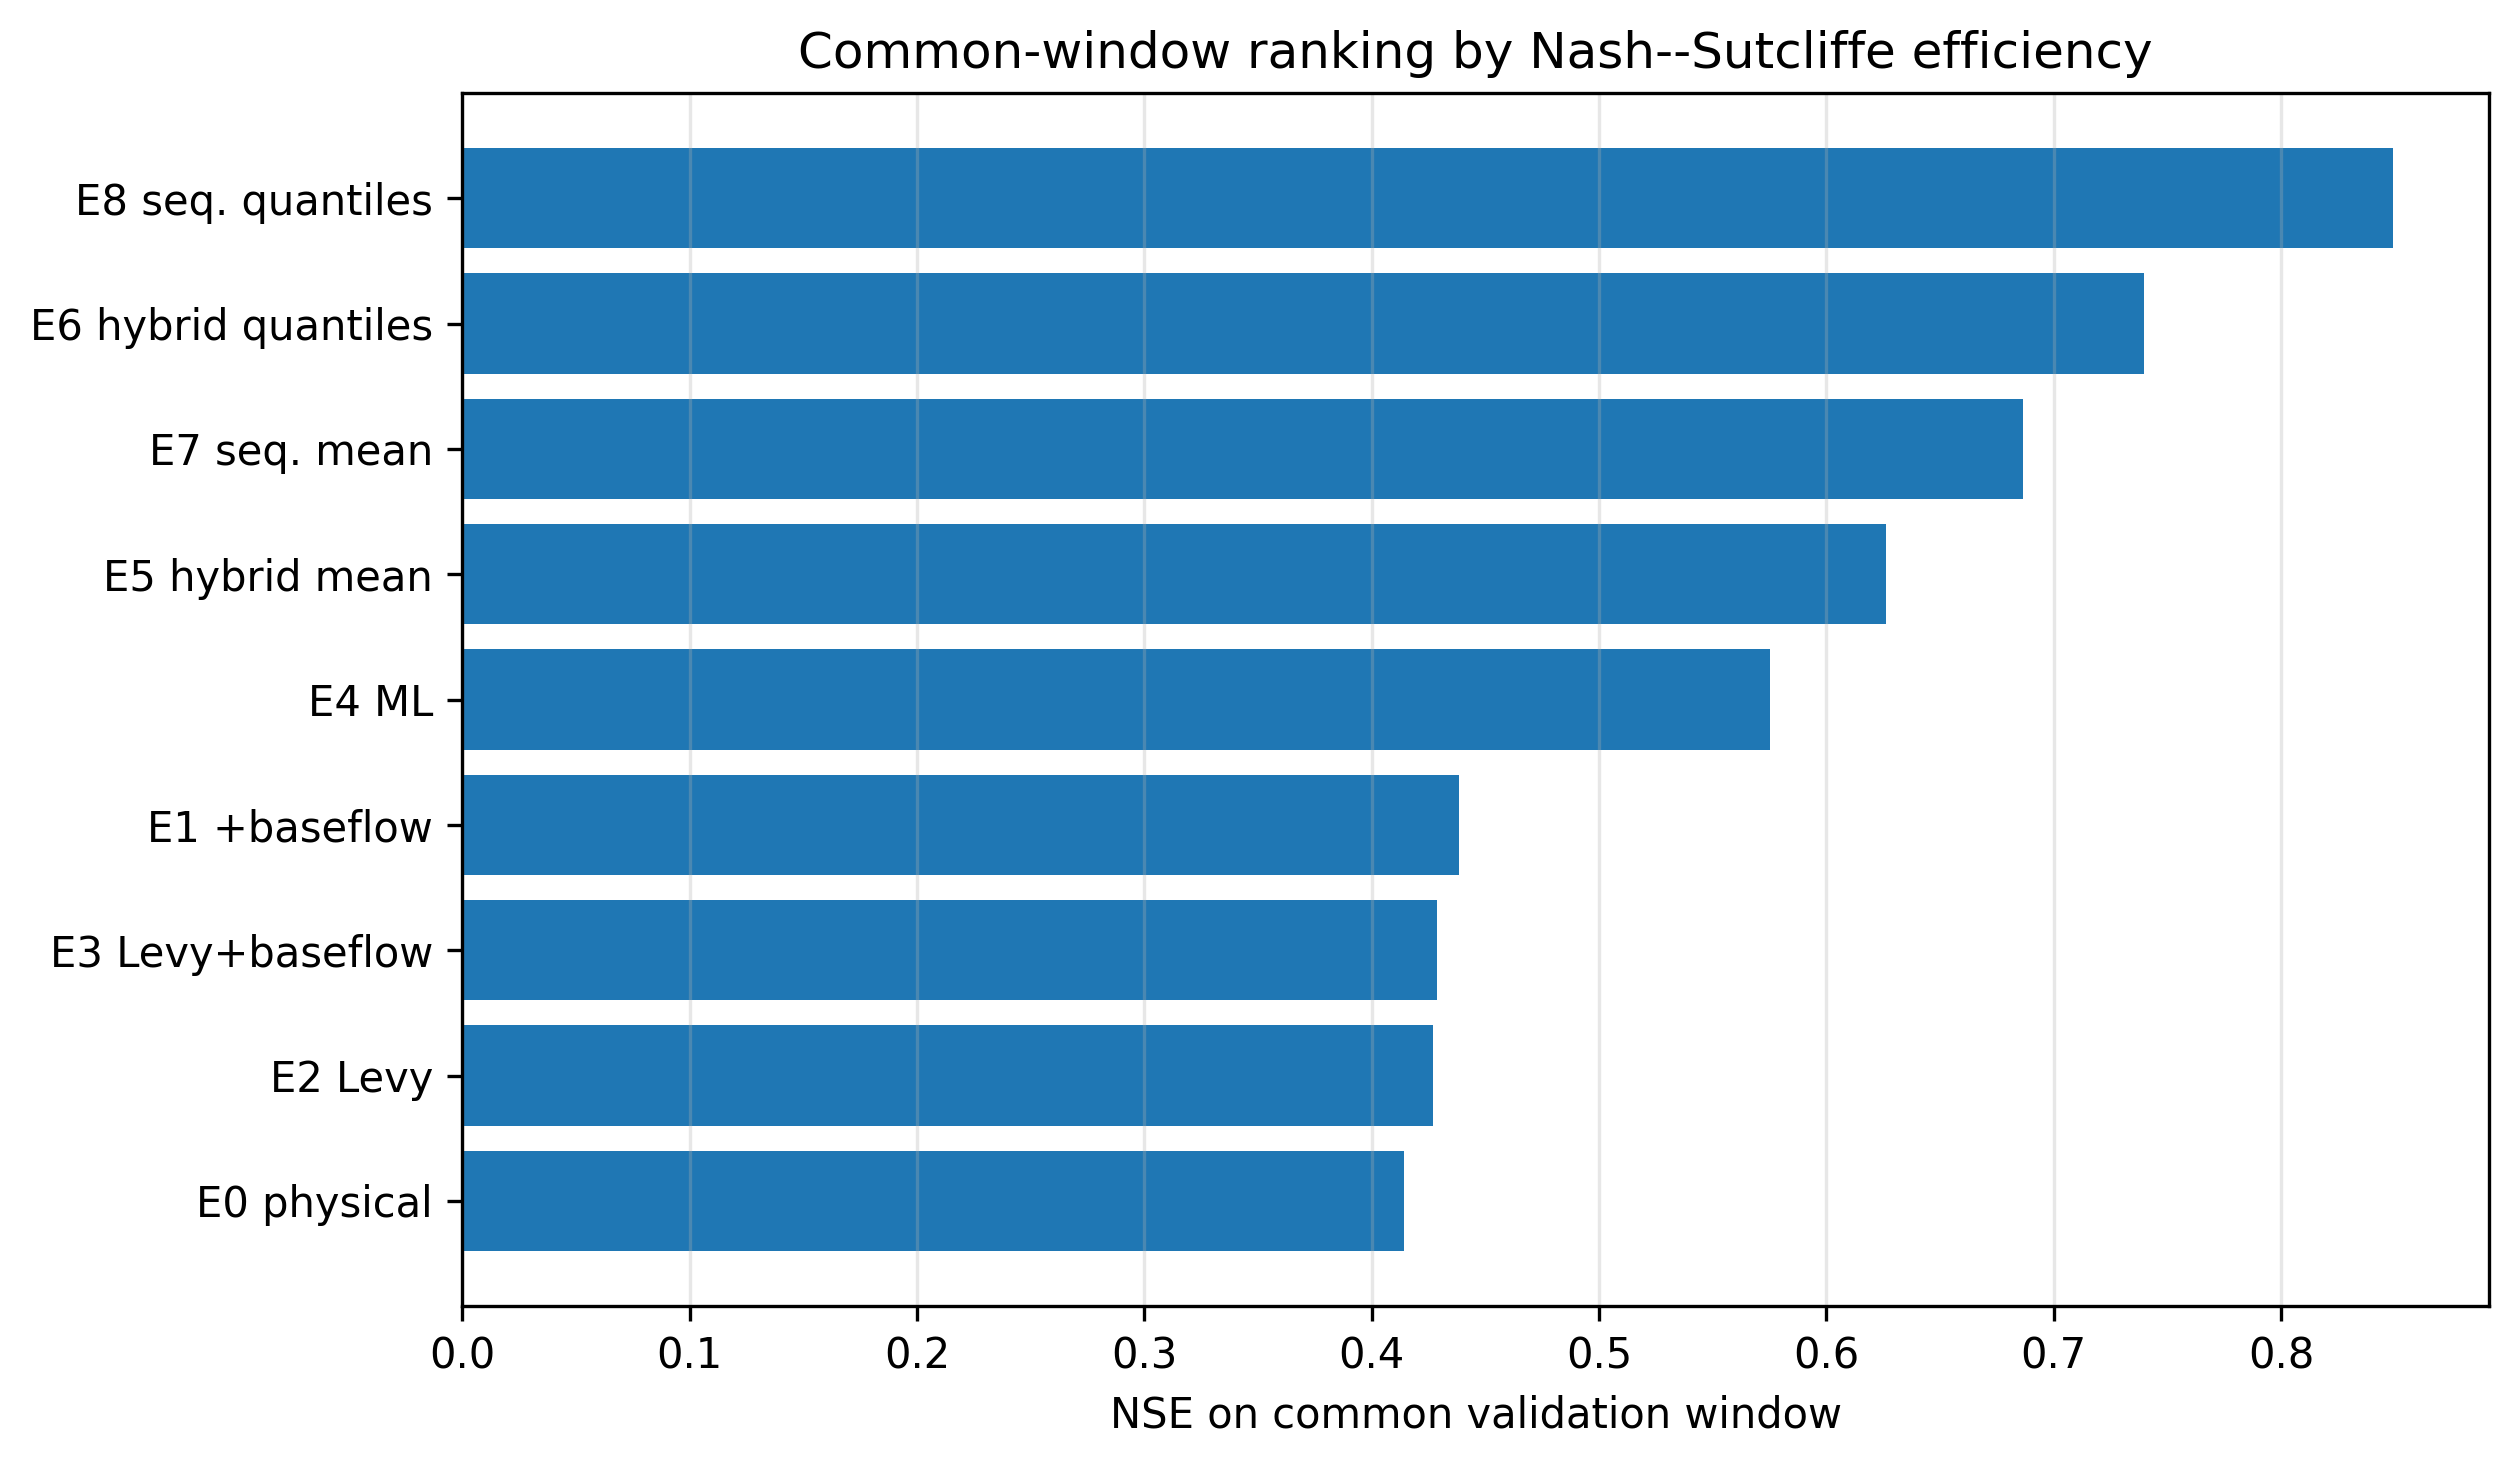
\includegraphics[width=0.95\linewidth]{figures/metric_ranking_nse.png}
\caption{Ranking of experiments by common-window NSE. Numerical values
correspond to Table~\ref{tab:ranking}; the GRU-labelled entries should
be interpreted with the backend audit because they executed as fallback
MLP models.}
\label{fig:metric-ranking}
\end{figure}

\subsection{Hydrograph and flow-duration behaviour}
\label{subsec:hydro-results}

The validation hydrograph in Fig.~\ref{fig:hydrograph-common} shows
that the hybrid models reproduce the timing and amplitude of seasonal
streamflow fluctuations more closely than the physical-only baselines.
The physical models retain the main wet-season response but frequently
collapse towards near-zero discharge during recession periods. This
behaviour is also evident in the flow-duration curves
(Fig.~\ref{fig:fdc-common}), where E0 shows an unrealistic decline in
the high-exceedance tail. Adding the baseflow reservoir reduces this
problem only partially, indicating that the single linear storage term
improves recession persistence but does not fully resolve dry-season
memory.

The hybrid configurations provide a closer match to the observed
flow-duration curve over most exceedance probabilities. The largest
visual improvement occurs in the lower-flow tail, where quantile-based
hybrids avoid the extreme collapse of the deterministic physical
trajectory. Nevertheless, the hydrograph also shows remaining errors
during sharp wet-season peaks. Thus, the hybrid improvement is not a
complete correction of event-scale dynamics; it is mainly a reduction
of systematic distributional errors and dry-season underestimation.

\begin{figure*}
\centering
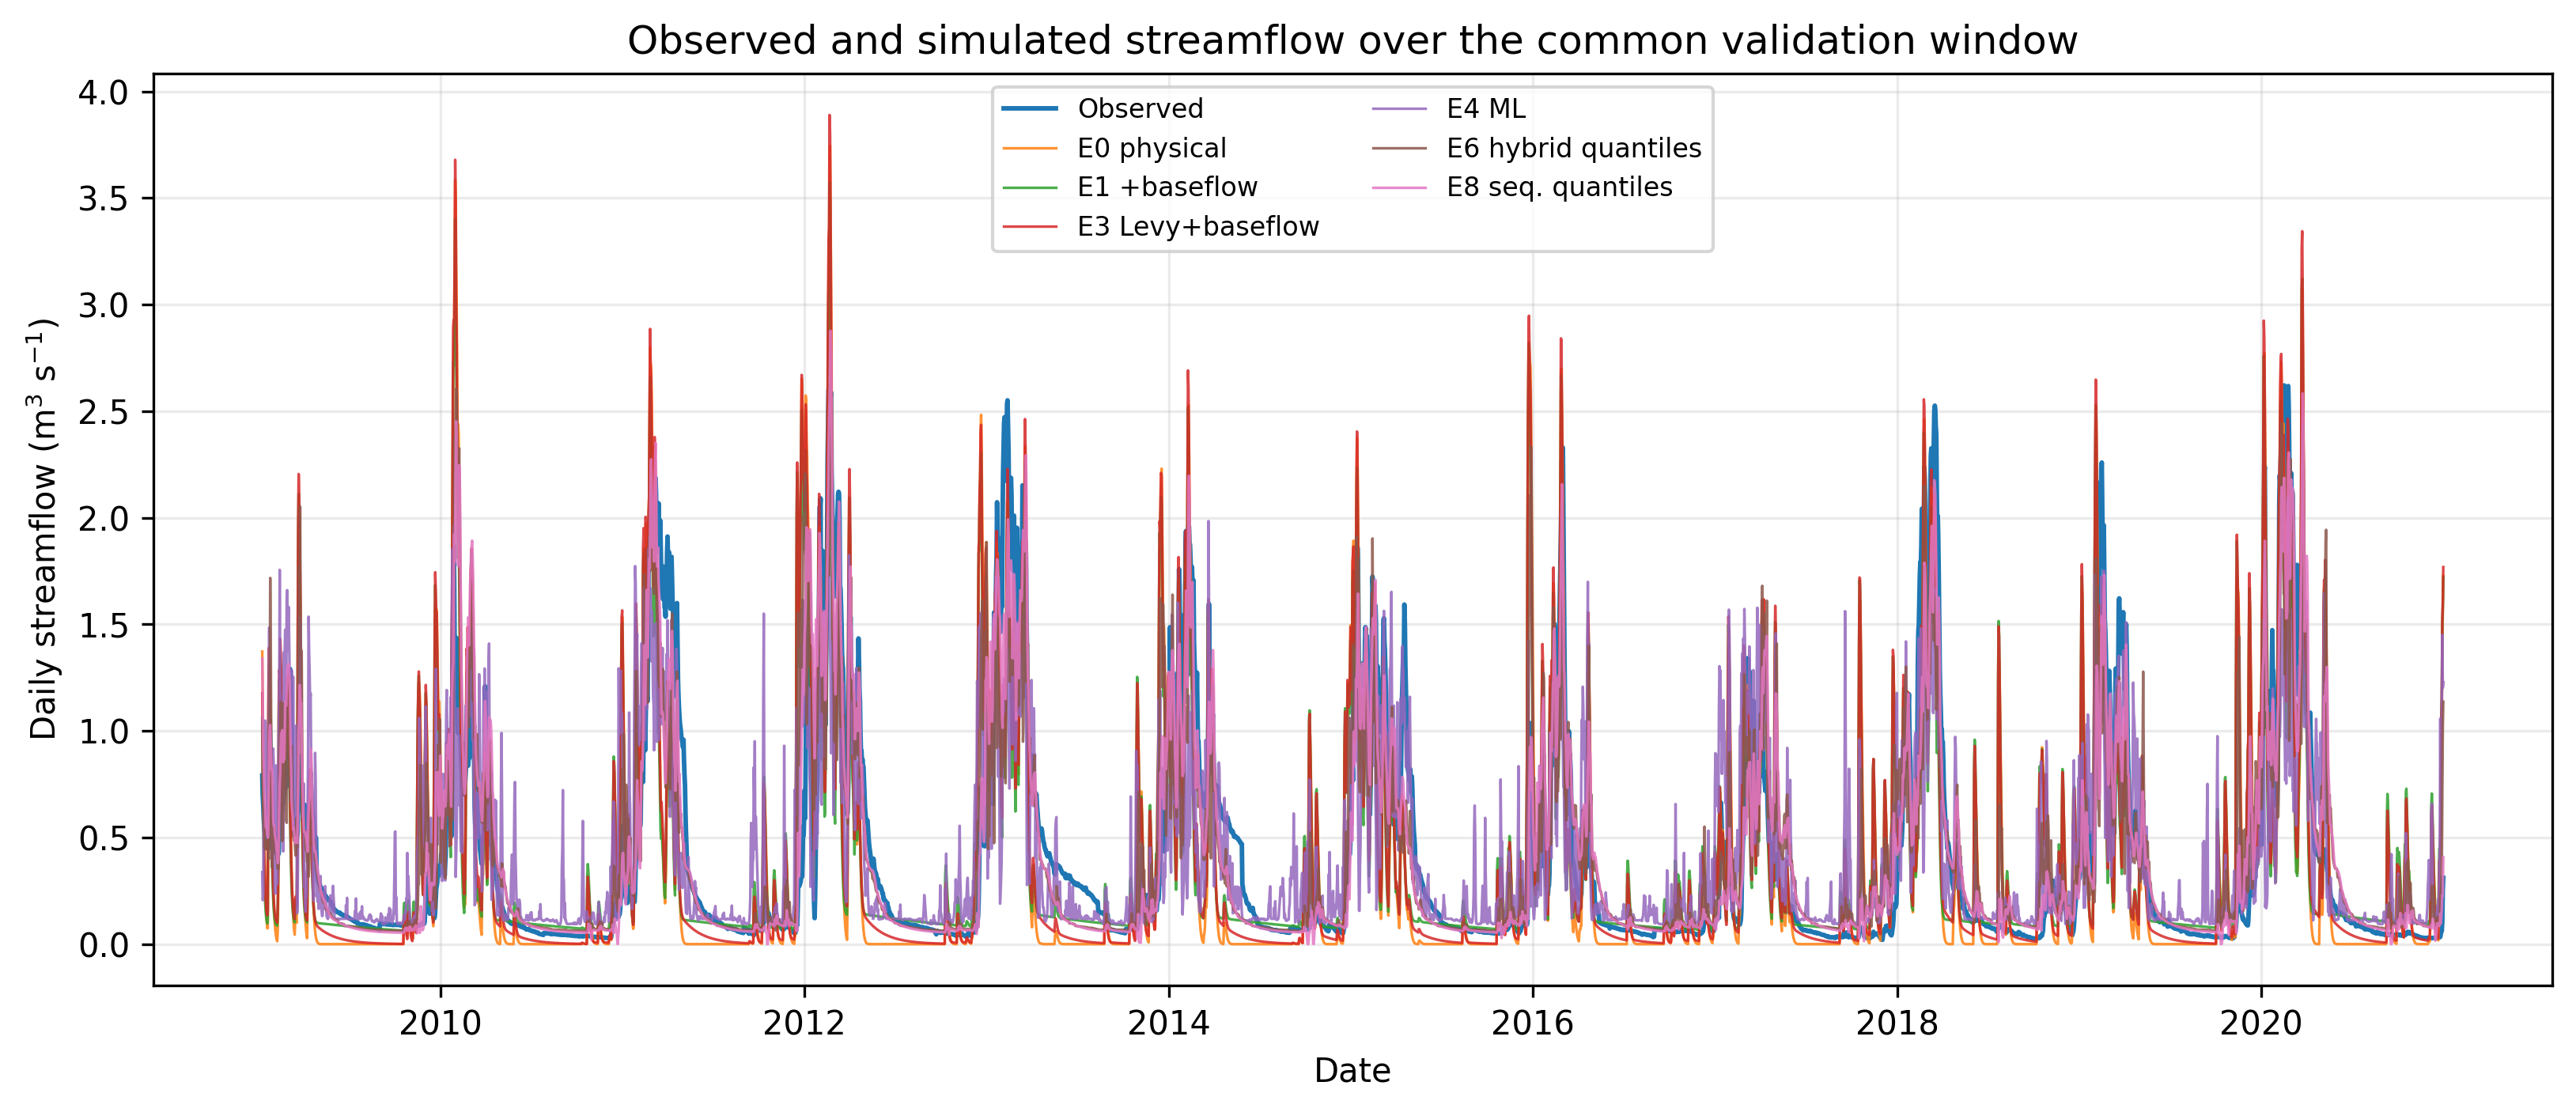
\includegraphics[width=0.98\textwidth]{figures/hydrograph_validation_common.png}
\caption{Observed and simulated daily discharge (\cms) over the common
validation window for representative physical, pure ML and hybrid
models.}
\label{fig:hydrograph-common}
\end{figure*}

\begin{figure}
\centering
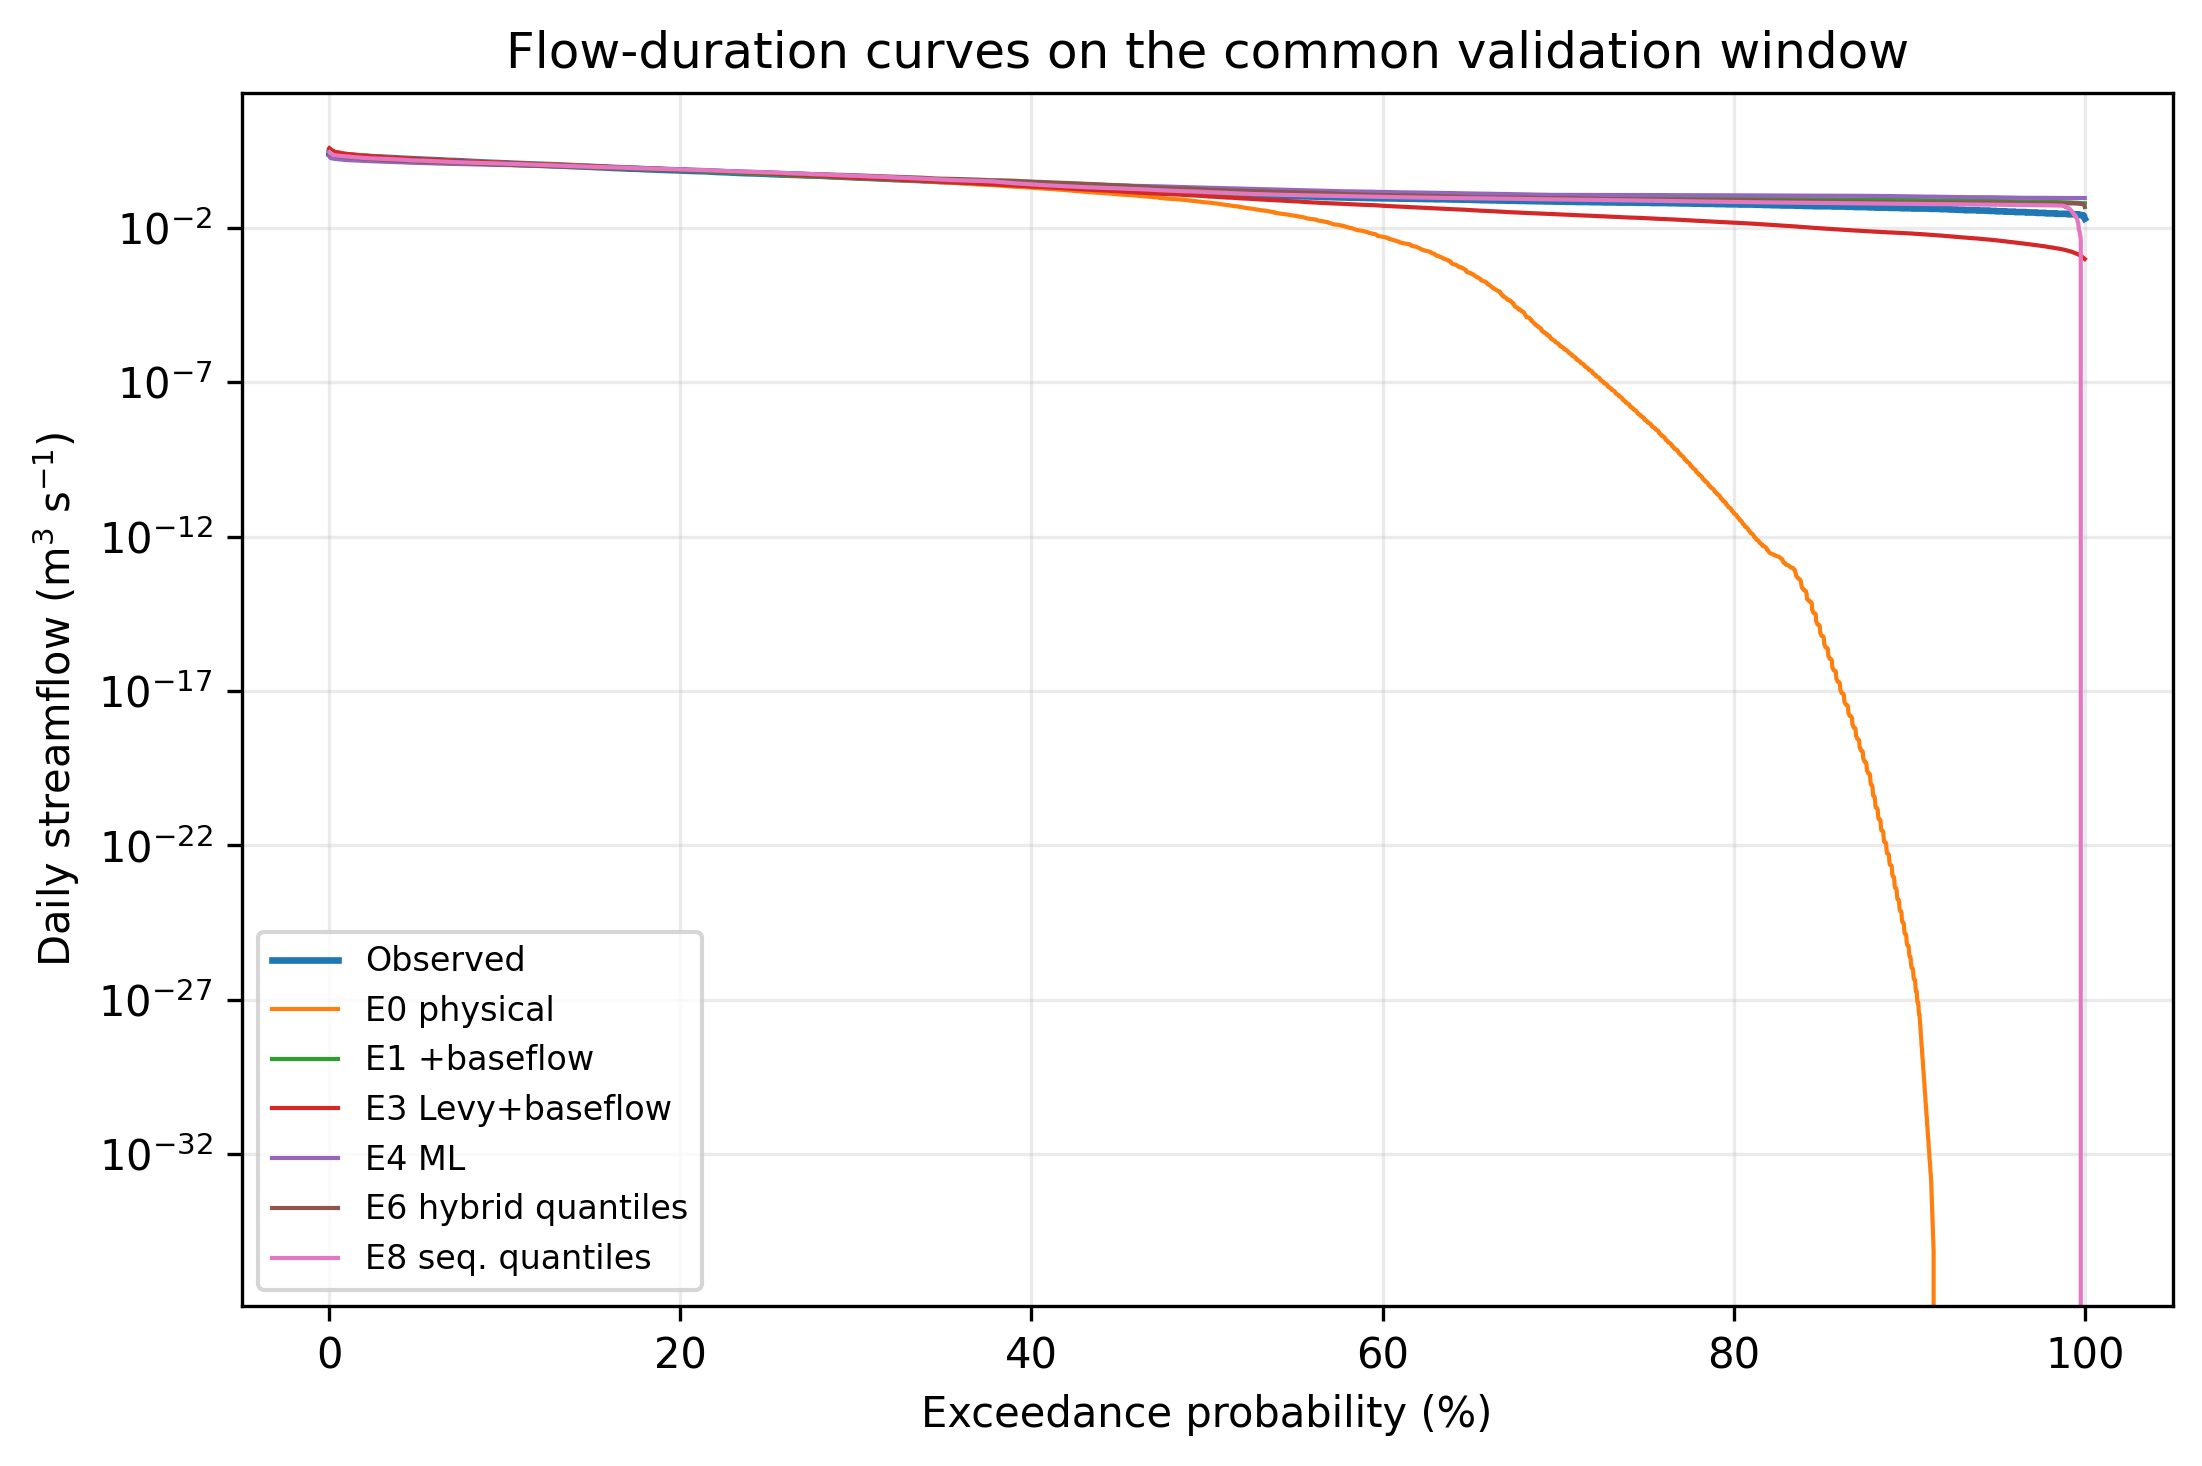
\includegraphics[width=0.95\linewidth]{figures/fdc_common.png}
\caption{Flow-duration curves for observed and simulated daily discharge
(\cms) over the common validation window.}
\label{fig:fdc-common}
\end{figure}

\subsection{Ablation effects}\label{subsec:ablation-results}

Table~\ref{tab:ablation} and Fig.~\ref{fig:ablation-effects} isolate
the contribution of each modelling component. Adding the baseflow
reservoir to the deterministic physical model increased NSE by 0.024
and reduced RMSE by 0.009~m$^3$\,s$^{-1}$ (E1--E0). Under stochastic
forcing, the same structural addition produced a smaller but still
positive gain in NSE and KGE (E3--E2). In contrast, adding
L\'{e}vy-type perturbations to the baseflow-enabled physical model did
not improve point-prediction skill: NSE decreased by 0.010 and RMSE
increased by 0.004~m$^3$\,s$^{-1}$, although KGE increased slightly.
This indicates that stochastic perturbation is not, by itself, the main
source of point-prediction improvement.

The largest gain came from hybridization. Relative to the complete
stochastic physical baseline (E3), the pure forcing-based ML model
(E4) improved NSE by 0.147, whereas the XGB-labelled hybrid using
ensemble means (E5) improved NSE by 0.198. The quantile-based hybrid
(E6) produced the largest backend-consistent ablation effect, with
$\Delta$NSE\,=\,0.311 and $\Delta$RMSE\,=\,-0.133~m$^3$\,s$^{-1}$
relative to E3. The direct comparison between E6 and E5 added
0.114 NSE and 0.095 KGE, showing that ensemble quantiles carry useful
predictive information that is lost when the stochastic physical
ensemble is compressed to its mean alone.

The GRU-labelled contrasts must be interpreted with the backend audit
in mind. E7 and E8 improved over their XGB-labelled counterparts, but
these gains cannot be attributed to recurrent-network memory because
both runs used a fallback MLP backend. They are therefore reported as
additional sequential-feature experiments under fallback execution, not
as evidence that GRU architecture is superior.


\begin{table*}
\caption{Component-wise ablation effects on the common validation window.
All values are candidate-minus-baseline differences; $\Delta$RMSE and
$\Delta$MAE are reported in \cms.}
\label{tab:ablation}
\centering
\scriptsize
\begin{tabularx}{\textwidth}{@{}>{\raggedright\arraybackslash}X>{\raggedright\arraybackslash}p{0.20\textwidth}>{\raggedright\arraybackslash}p{0.21\textwidth}rrrr@{}}
\toprule
Ablation & Baseline & Candidate
  & $\Delta$NSE & $\Delta$KGE & $\Delta$RMSE (\cms) & $\Delta$MAE (\cms) \\
\midrule
deterministic baseflow
  & \modelid{E0_RAMIS_DET_NOBF} & \modelid{E1_RAMIS_DET_BF}
  & 0.024 & 0.000 & -0.009 & -0.022 \\
stochastic baseflow
  & \modelid{E2_RAMIS_LEVY_NOBF} & \modelid{E3_RAMIS_LEVY_BF}
  & 0.002 & 0.008 & -0.001 & -0.012 \\
L\'{e}vy given baseflow
  & \modelid{E1_RAMIS_DET_BF} & \modelid{E3_RAMIS_LEVY_BF}
  & -0.010 & 0.011 & 0.004 & 0.008 \\
pure ML vs physical
  & \modelid{E3_RAMIS_LEVY_BF} & \modelid{E4_ML_PURE_XGB}
  & 0.147 & -0.064 & -0.056 & -0.033 \\
hybrid mean vs physical
  & \modelid{E3_RAMIS_LEVY_BF} & \modelid{E5_HYB_XGB_MEAN}
  & 0.198 & -0.010 & -0.078 & -0.046 \\
hybrid quantiles vs physical
  & \modelid{E3_RAMIS_LEVY_BF} & \modelid{E6_HYB_XGB_QUANTILES}
  & 0.311 & 0.085 & -0.133 & -0.094 \\
quantiles vs mean, HGB
  & \modelid{E5_HYB_XGB_MEAN} & \modelid{E6_HYB_XGB_QUANTILES}
  & 0.114 & 0.095 & -0.055 & -0.048 \\
sequence mean vs HGB mean
  & \modelid{E5_HYB_XGB_MEAN} & \modelid{E7_HYB_GRU_MEAN}
  & 0.060 & 0.074 & -0.028 & -0.018 \\
sequence quantiles vs HGB quantiles
  & \modelid{E6_HYB_XGB_QUANTILES} & \modelid{E8_HYB_GRU_QUANTILES}
  & 0.109 & 0.089 & -0.066 & -0.038 \\
\bottomrule
\end{tabularx}
\end{table*}

\begin{figure}
\centering
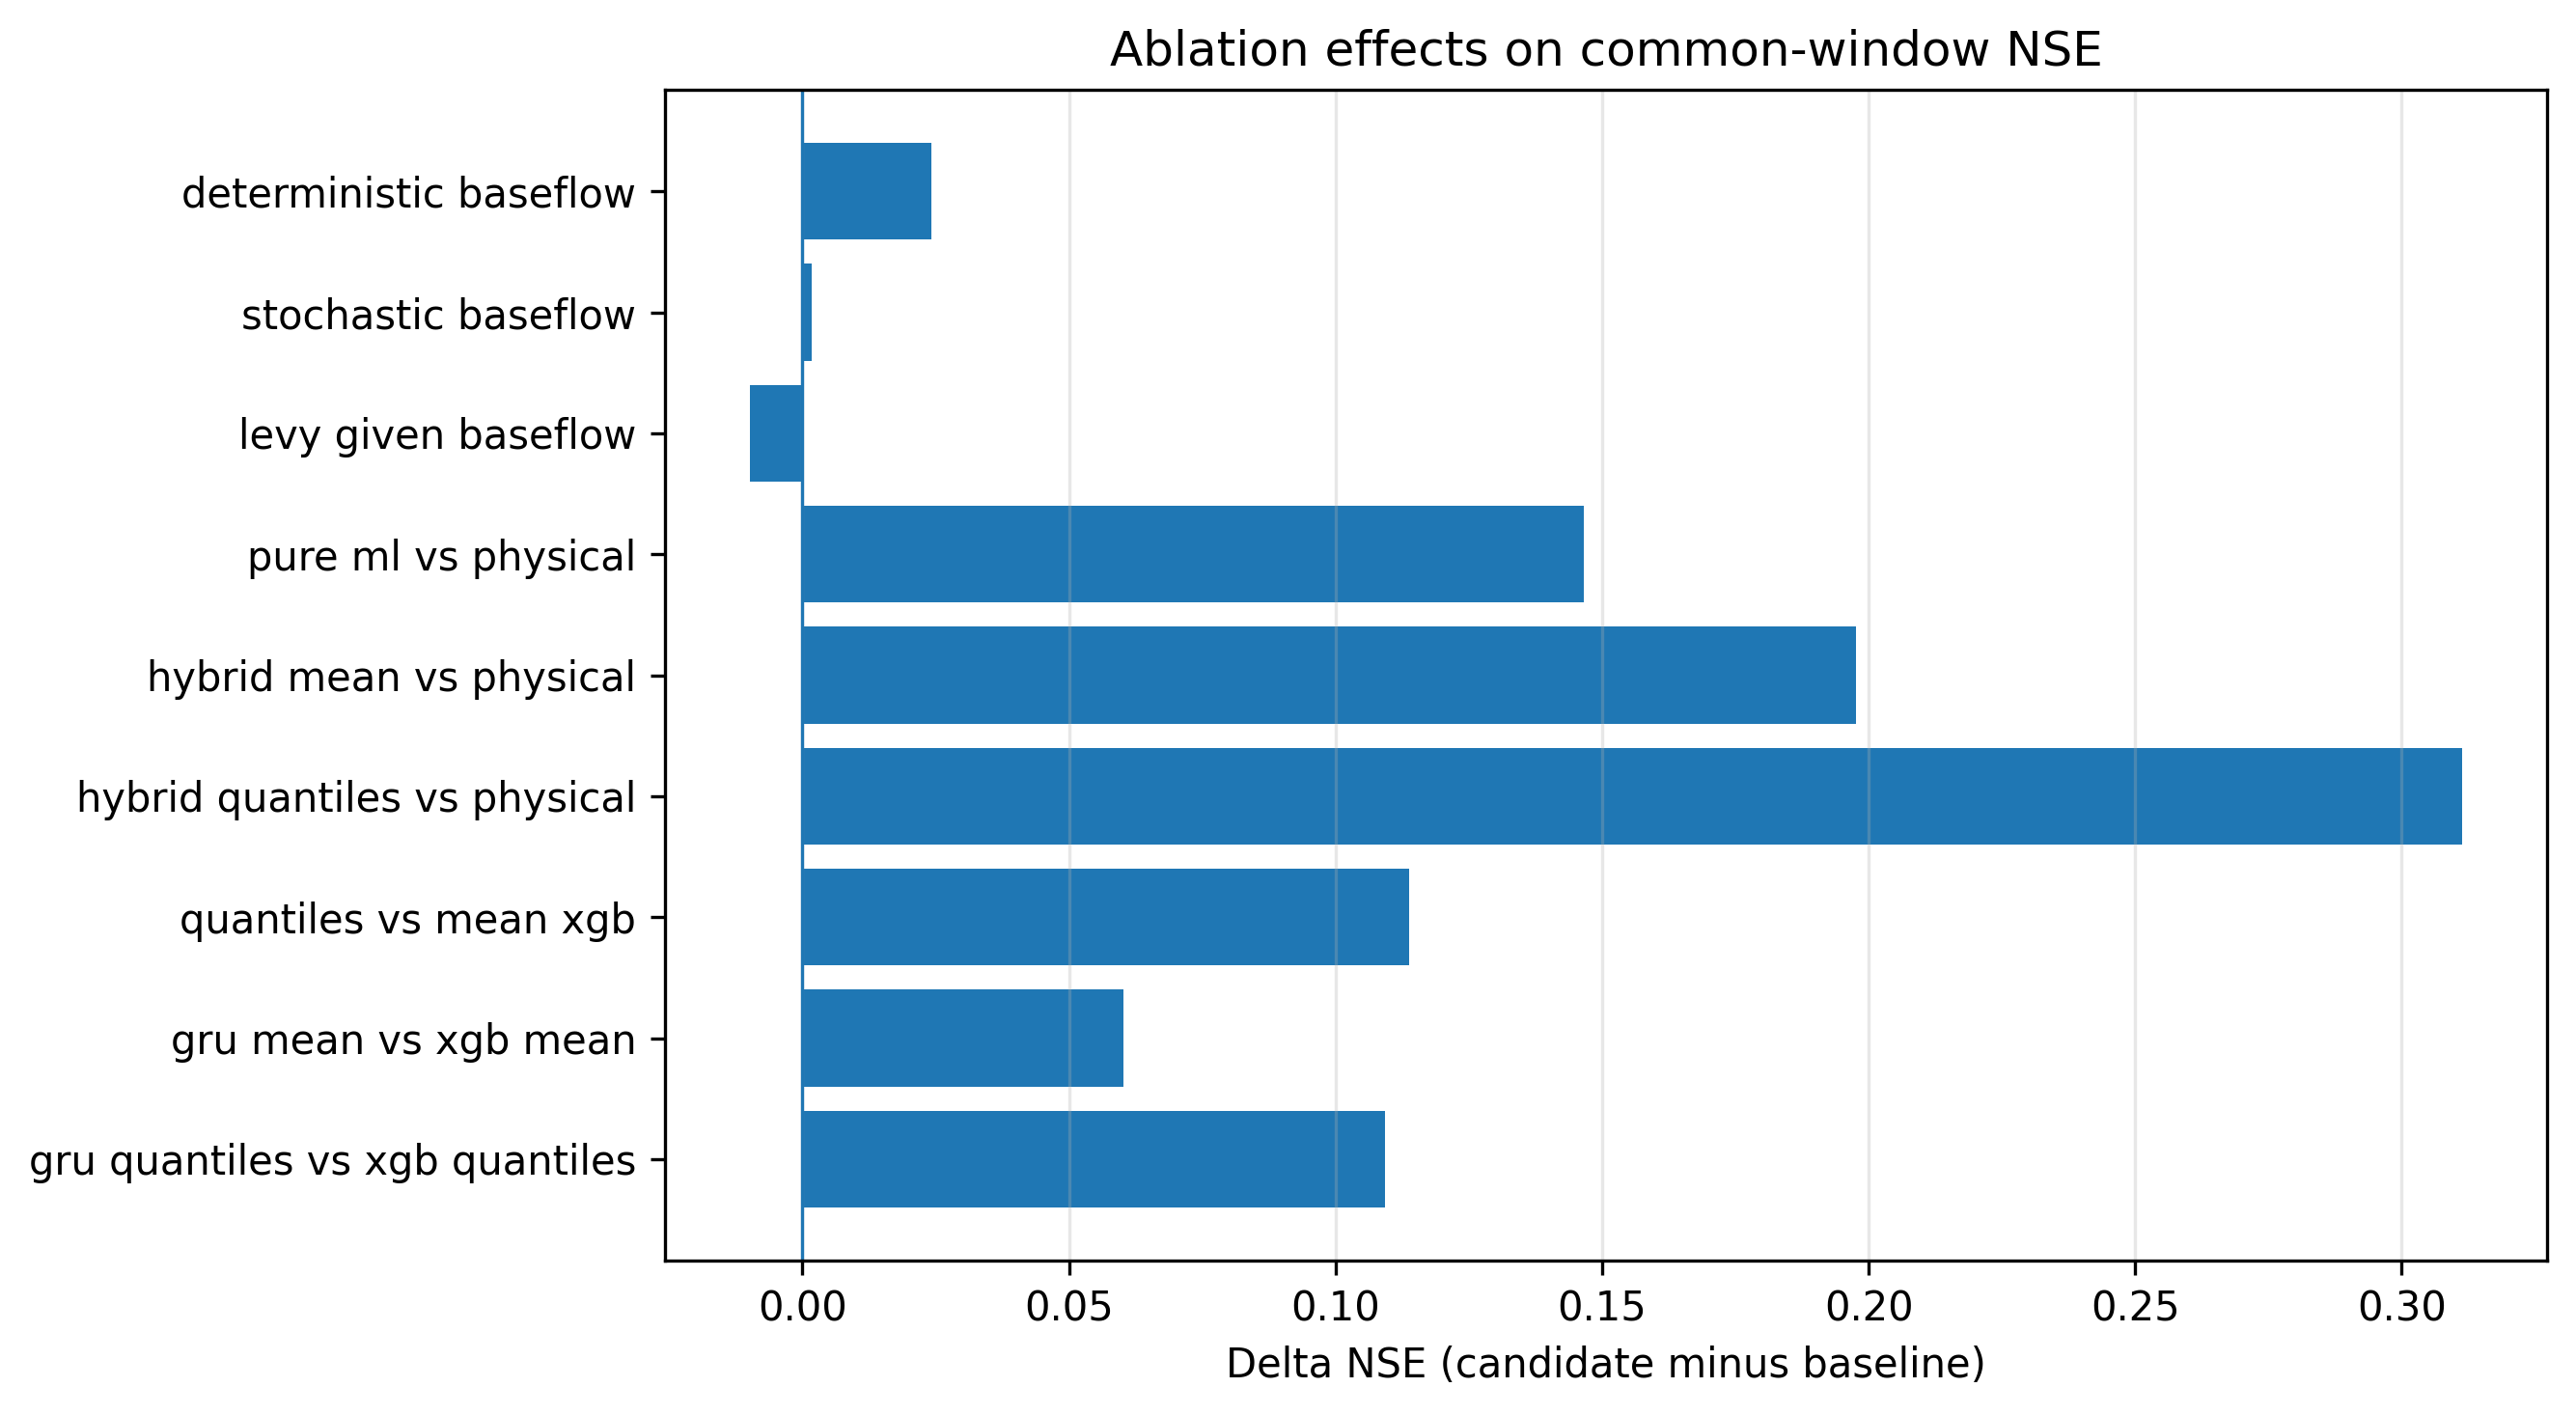
\includegraphics[width=0.95\linewidth]{figures/ablation_effects.png}
\caption{Ablation effects expressed as candidate-minus-baseline
$\Delta$NSE. Numerical values are reported in Table~\ref{tab:ablation};
GRU-labelled contrasts refer to fallback-MLP execution in the current
analysis archive.}
\label{fig:ablation-effects}
\end{figure}

\subsection{Performance by flow regime}\label{subsec:regime-results}

Regime-specific RMSE values (Table~\ref{tab:regime-rmse} and
Fig.~\ref{fig:regime-rmse}) show that model skill is strongly
flow-dependent. The physical-only configurations had similar errors
across the selected regimes, with the largest absolute errors in the
high-flow class. The pure ML model reduced mid-flow RMSE relative to
the physical baselines, but its low-flow RMSE remained close to that of
the physical models. The quantile-based hybrid E6 reduced
errors in all regimes, and the numerically best E8 configuration
further reduced RMSE under fallback-MLP execution.

The largest proportional improvement occurred in the low-flow regime:
RMSE decreased from 0.177~m$^3$\,s$^{-1}$ for E0 to
0.075~m$^3$\,s$^{-1}$ for E6 and 0.047~m$^3$\,s$^{-1}$ for E8. The
mid-flow and high-flow regimes also improved, but larger residual
errors persisted during high flows, where event timing and peak
magnitude remain more difficult to reproduce. These results support the
interpretation from the flow-duration curves: stochastic ensemble
quantiles are most useful for correcting systematic distributional
errors, especially during recession and low-flow periods, while peak
simulation remains only partially corrected.


\begin{table}
\caption{RMSE (\cms) by flow regime for representative models. Regime
thresholds were estimated from calibration observations only.}
\label{tab:regime-rmse}
\centering
\footnotesize
\begin{tabularx}{\linewidth}{@{}>{\raggedright\arraybackslash}Xrrr@{}}
\toprule
Experiment & Low & Mid & High \\
\midrule
\modelid{E0_RAMIS_DET_NOBF}    & 0.177 & 0.392 & 0.615 \\
\modelid{E1_RAMIS_DET_BF}      & 0.197 & 0.365 & 0.613 \\
\modelid{E3_RAMIS_LEVY_BF}     & 0.185 & 0.387 & 0.604 \\
\modelid{E4_ML_PURE_XGB}       & 0.189 & 0.276 & 0.566 \\
\modelid{E6_HYB_XGB_QUANTILES} & 0.075 & 0.222 & 0.461 \\
\modelid{E8_HYB_GRU_QUANTILES} & 0.047 & 0.171 & 0.352 \\
\bottomrule
\end{tabularx}
\end{table}

\begin{figure}
\centering
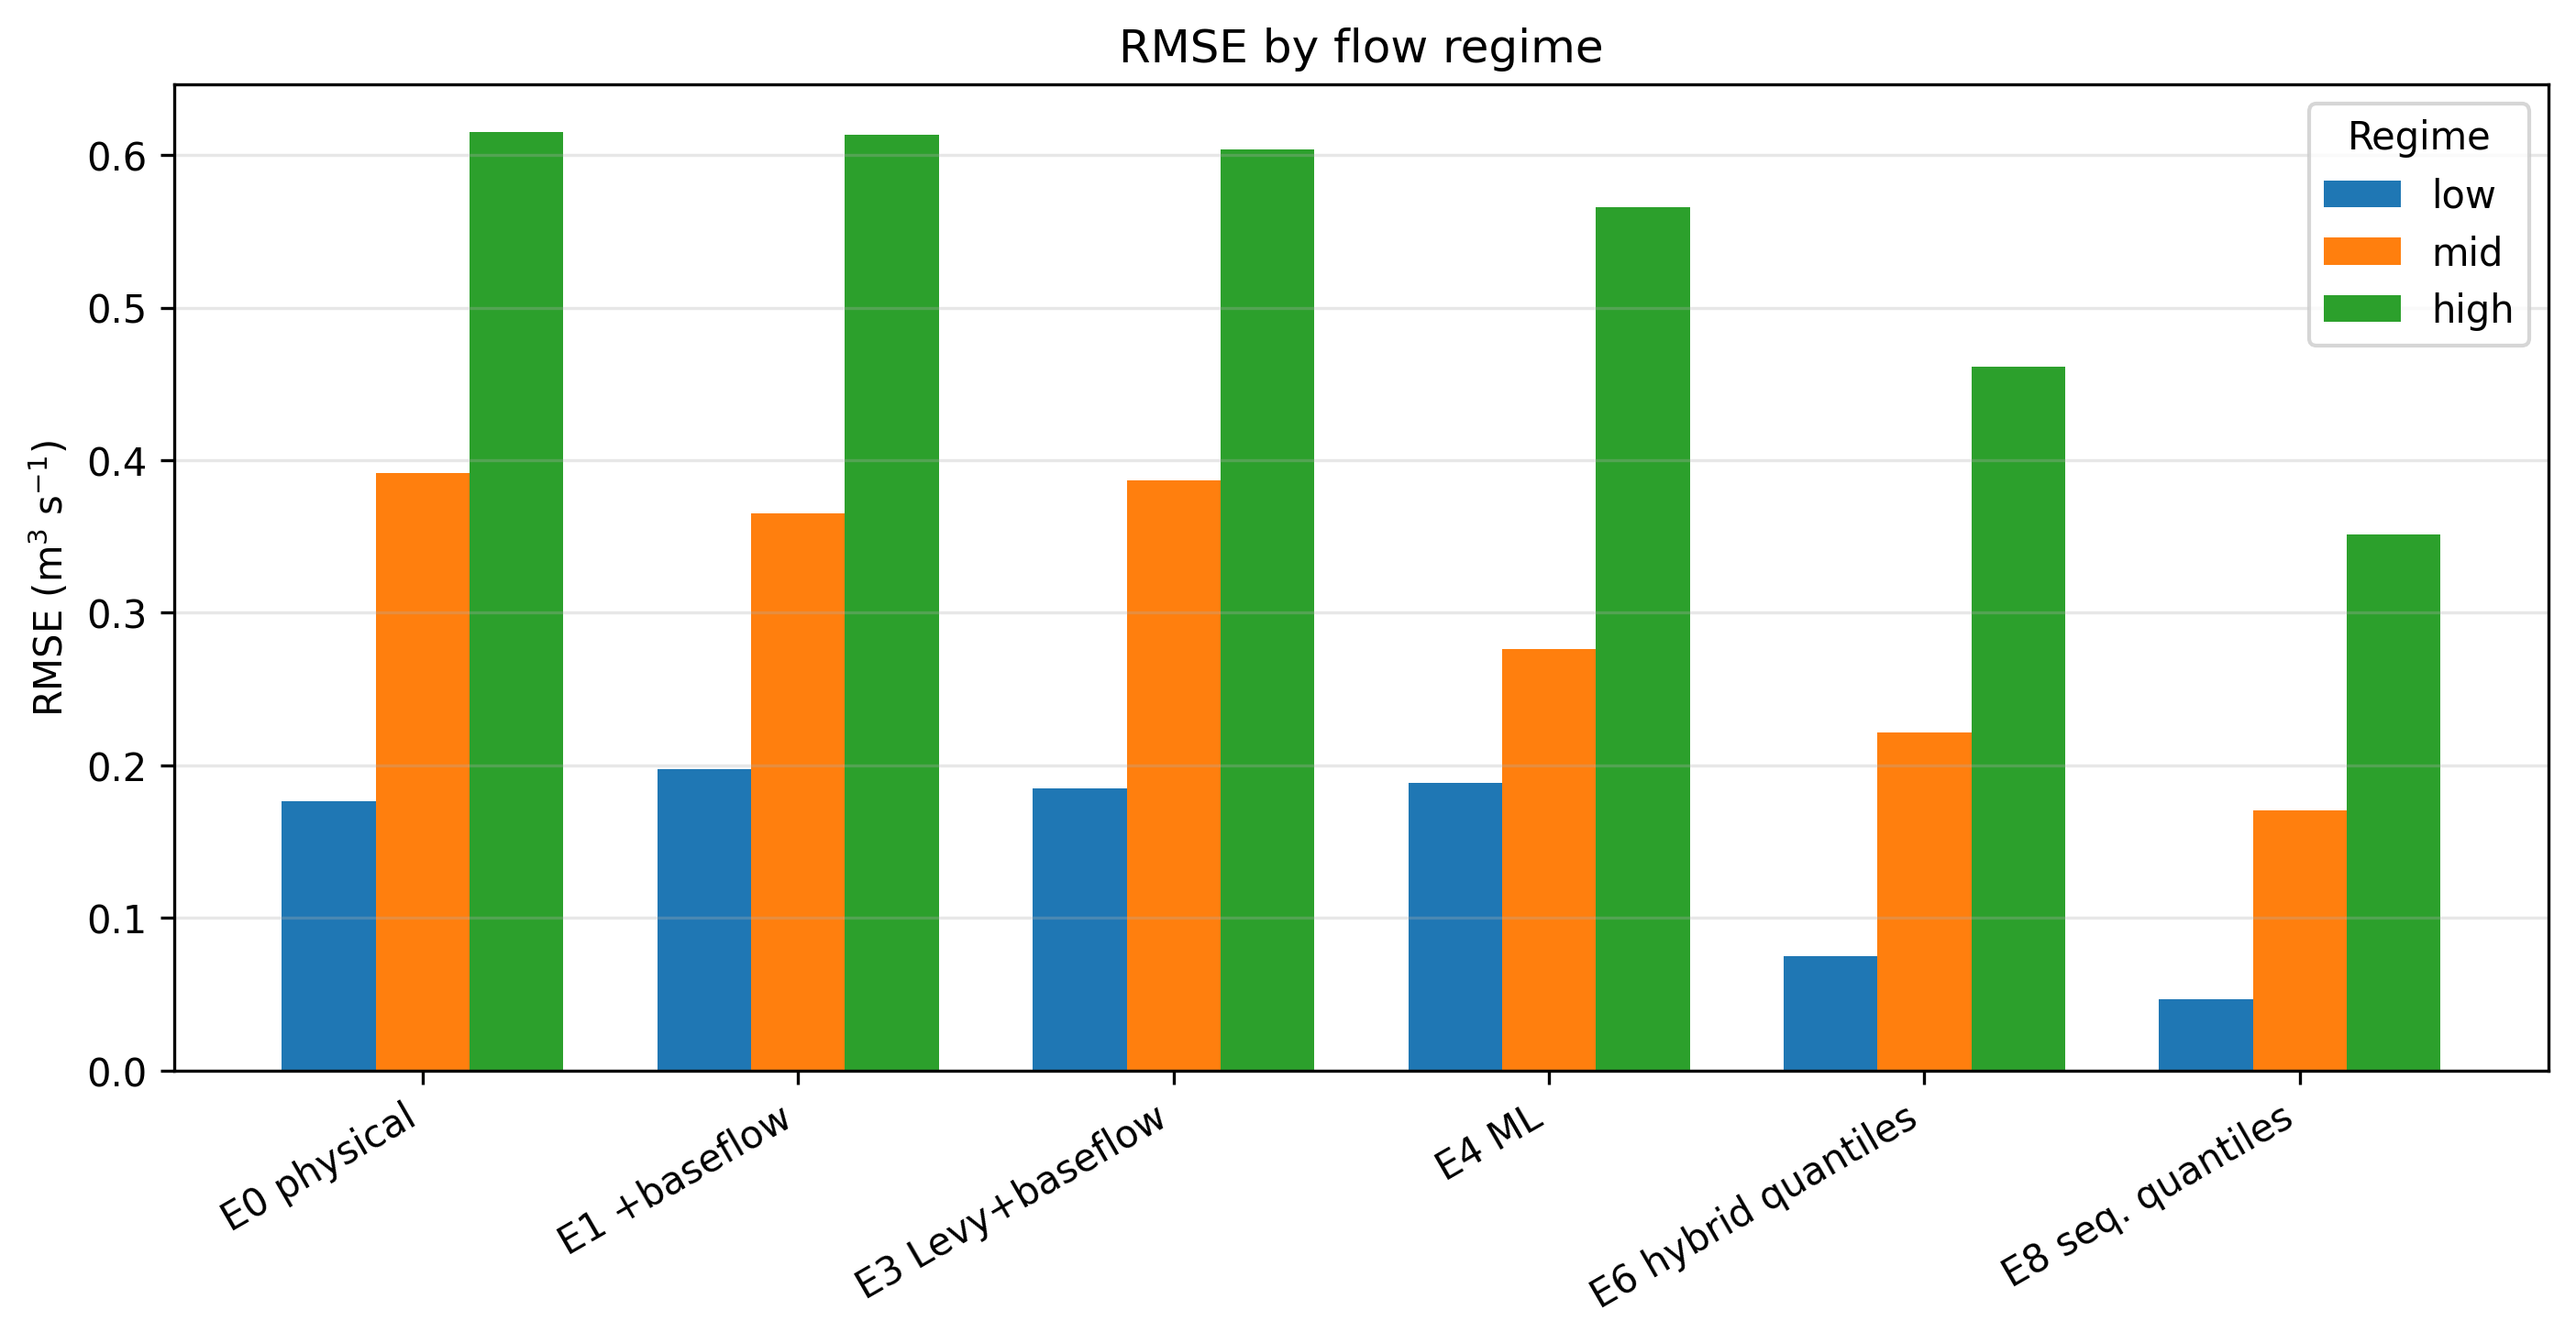
\includegraphics[width=0.95\linewidth]{figures/regime_rmse.png}
\caption{RMSE (\cms) by low-, mid- and high-flow regimes for representative
models. Values correspond to Table~\ref{tab:regime-rmse}.}
\label{fig:regime-rmse}
\end{figure}

\subsection{Uncertainty diagnostics and backend audit}
\label{subsec:uncertainty-results}

The stochastic physical intervals were strongly underdispersive
(Table~\ref{tab:uncertainty} and Fig.~\ref{fig:uncertainty-diagnostics}).
E2 achieved PICP\,=\,0.160 and E3 achieved PICP\,=\,0.004, both far
below the nominal 0.95 target. The corresponding PINAW values were also
small, particularly for E3 (PINAW\,=\,0.003), indicating that the
intervals were narrow rather than reliably calibrated. The high Winkler
scores indicate that most observed values fell outside the nominal
intervals. Consequently, the stochastic ensemble should not be reported
as a calibrated predictive uncertainty product in its current form. Its
main demonstrated value is as a source of physically structured
features for ML correction.

Table~\ref{tab:backend} summarizes the backend audit. The XGB-labelled
experiments (E4--E6) used the \texttt{sklearn\_hgb} backend, whereas
the GRU-labelled experiments (E7 and E8) used
\texttt{fallback\_mlp\_on\_flattened\_sequences}. This distinction
changes the interpretation of the leaderboard: E8 may be reported as
the best numerical experiment, but not as evidence for recurrent neural
networks. The reproducibility checklist in
Table~\ref{tab:reproducibility} returned no FAIL item. WARN items were
associated with missing observed-flow values, low-flow physical
limitations, optional figure entries and the fallback backend, rather
than with direct evidence of temporal leakage.


\begin{table}
\caption{Uncertainty diagnostics for stochastic physical reference bands.
PICP and PINAW are dimensionless; MPIW and Winkler score are reported in
\cms.}
\label{tab:uncertainty}
\centering
\footnotesize
\begin{tabularx}{\linewidth}{@{}>{\raggedright\arraybackslash}Xrrrr@{}}
\toprule
Experiment & PICP & PINAW & MPIW (\cms) & Winkler (\cms) \\
\midrule
\modelid{E2_RAMIS_LEVY_NOBF} & 0.160 & 0.084 & 0.219 & 7.297 \\
\modelid{E3_RAMIS_LEVY_BF}   & 0.004 & 0.003 & 0.009 & 10.050 \\
\bottomrule
\end{tabularx}
\end{table}

\begin{figure}
\centering
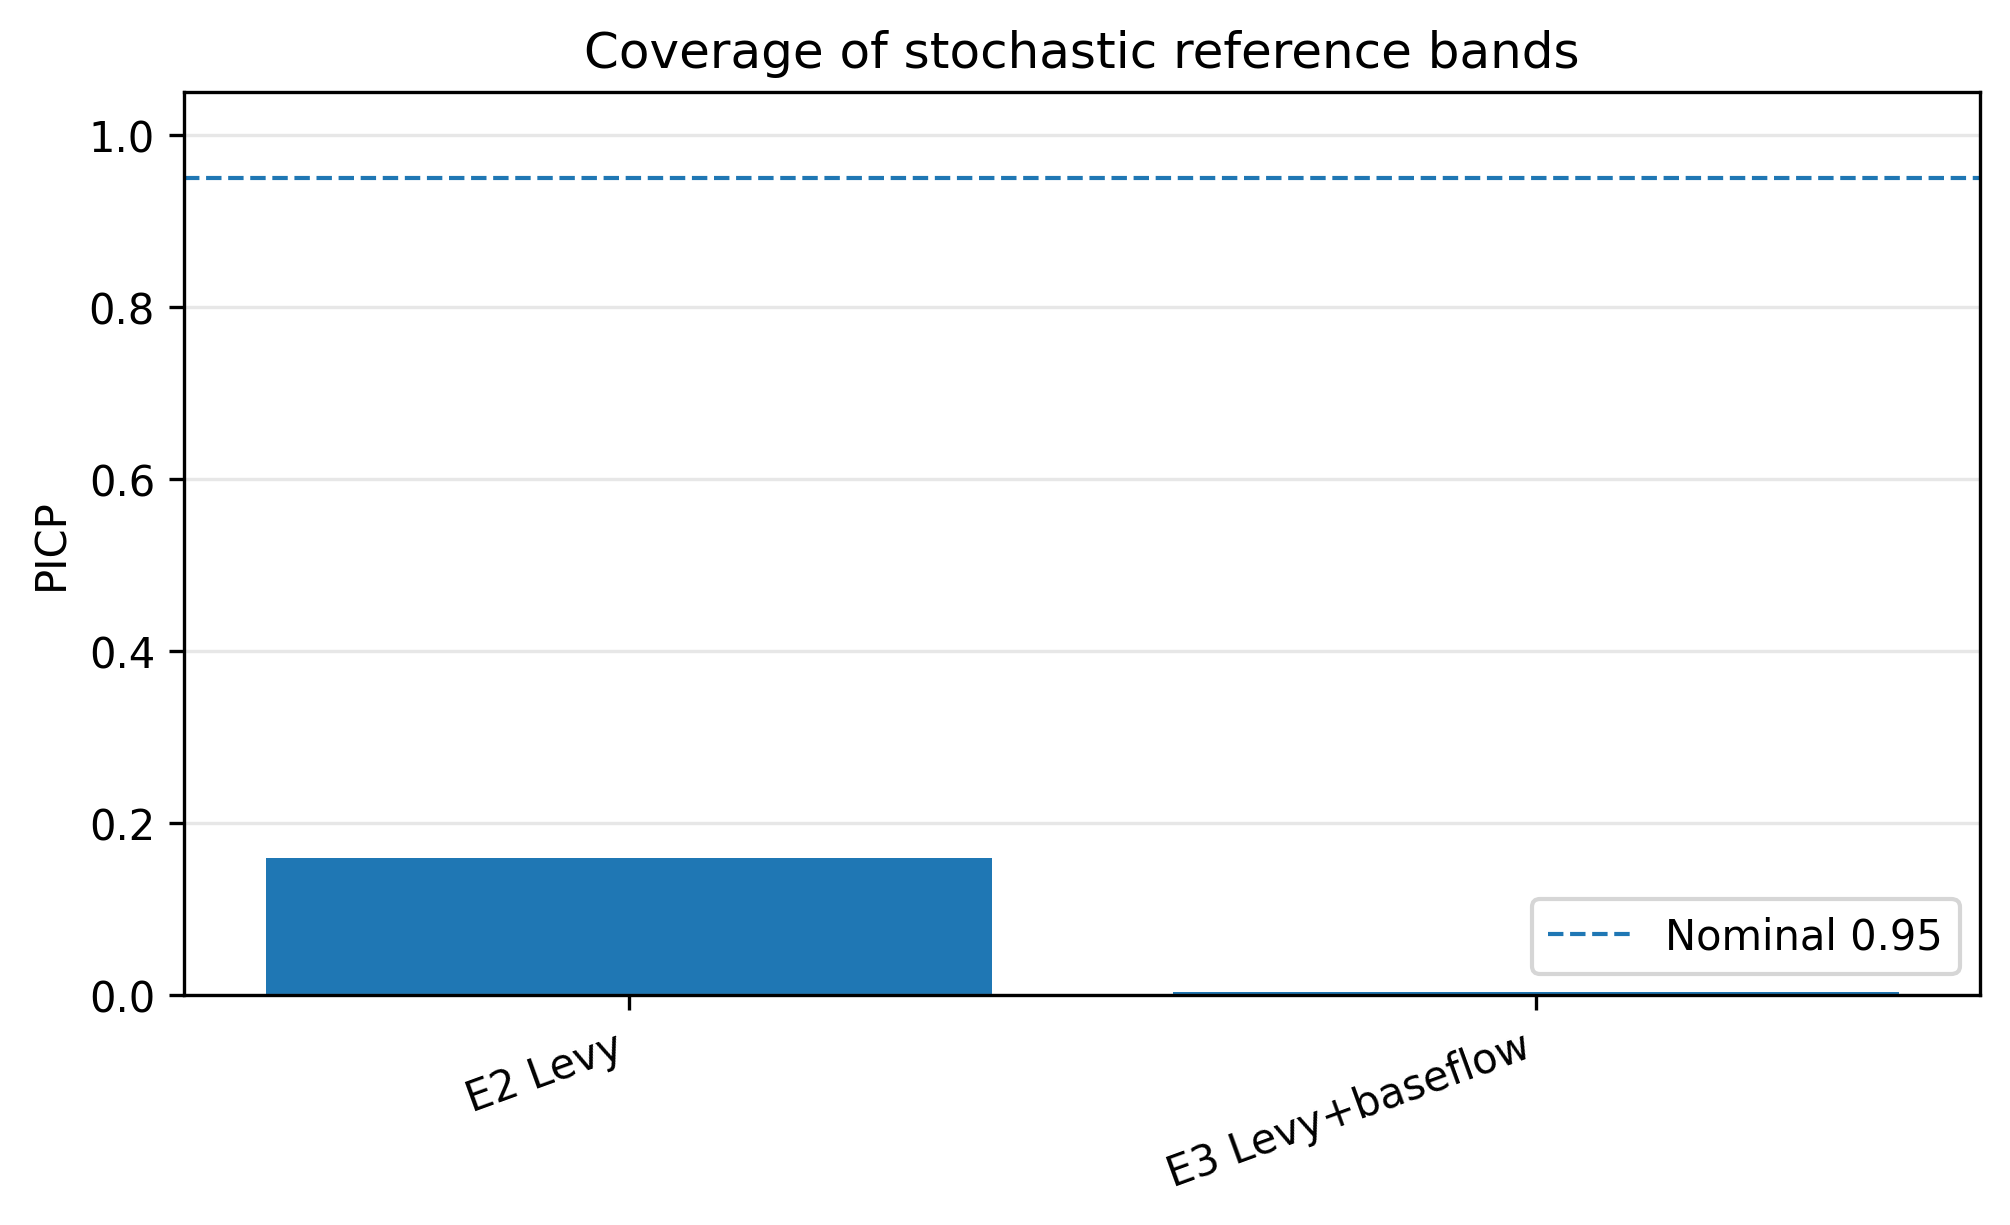
\includegraphics[width=0.95\linewidth]{figures/uncertainty_diagnostics.png}
\caption{Prediction interval coverage probability for nominal 95\% stochastic
physical reference intervals. The dashed line marks the nominal 0.95
coverage target.}
\label{fig:uncertainty-diagnostics}
\end{figure}


\begin{table*}
\caption{Backend-aware audit notes for ML and hybrid configurations. The
claim column states wording supported by the executed backend.}
\label{tab:backend}
\centering
\footnotesize
\begin{tabularx}{\textwidth}{@{}>{\raggedright\arraybackslash}p{0.23\textwidth}ll>{\raggedright\arraybackslash}X>{\raggedright\arraybackslash}p{0.24\textwidth}@{}}
\toprule
Experiment & ML label & Executed backend & Feature source
  & Supported manuscript wording \\
\midrule
\modelid{E4_ML_PURE_XGB}       & xgboost & HGB & observed forcings
  & gradient boosting; not library-specific XGBoost \\
\modelid{E6_HYB_XGB_QUANTILES} & xgboost & HGB & stochastic ensemble
  & gradient-boosting quantile hybrid \\
\modelid{E7_HYB_GRU_MEAN}      & gru & fallback MLP
  & stochastic ensemble & fallback MLP; not real recurrent GRU \\
\modelid{E8_HYB_GRU_QUANTILES} & gru & fallback MLP
  & stochastic ensemble & fallback MLP; not real recurrent GRU \\
\bottomrule
\end{tabularx}
\end{table*}


\begin{table*}
\caption{Reproducibility checklist for the current analysis archive. WARN
items identify issues to report or verify; they are not interpreted as
failures unless direct evidence of leakage is present.}
\label{tab:reproducibility}
\centering
\footnotesize
\begin{tabularx}{\textwidth}{@{}>{\raggedright\arraybackslash}p{0.30\textwidth}l>{\raggedright\arraybackslash}X@{}}
\toprule
Item & Status & Evidence \\
\midrule
Common validation intersection & PASS
  & All experiments evaluated on the same 4367-day validation window \\
Anti-leakage audit & WARN
  & Temporal ordering preserved; residual warning retained for transparent reporting \\
Physical audit   & WARN
  & Non-negative discharge and physical post-processing verified; optional components flagged where applicable \\
Figure consistency  & PASS
  & Figures and tables use the common validation window and the same experiment labels \\
GRU wording      & WARN
  & E7/E8 use fallback MLP execution rather than a verified recurrent backend \\
Optional physical components in figures & WARN
  & Optional physical components retained only where directly supported by the experiment matrix \\
\bottomrule
\end{tabularx}
\end{table*}


%% =====================================================================
%% 4. DISCUSSION
%% =====================================================================

\section{Discussion}\label{sec:discussion}

\subsection{Main inference from the ablation}
\label{subsec:discussion-main-inference}

The ablation results indicate that the principal source of improvement
is not stochastic perturbation alone, nor the nominal complexity of the
ML backend, but the transfer of distributional information from the
stochastic physical ensemble to the emulator. This distinction is
important for interpreting the experiment hierarchy. The deterministic
and stochastic physical baselines remain within a narrow performance
range, and direct L\'{e}vy perturbation of the baseflow-enabled physical
model does not improve point-prediction skill. By contrast, the
backend-consistent quantile hybrid E6 improves NSE by 0.311 relative to
the full stochastic physical baseline E3 and by 0.165 relative to the
pure forcing-based ML baseline E4. The most direct descriptor ablation,
E6--E5, adds 0.114 NSE by replacing an ensemble-mean feature with a
vector of ensemble quantiles while preserving the same executed
backend. This result supports a specific interpretation of hybridization:
the physical model is most useful when it is used to construct
informative state-dependent predictors, rather than when its stochastic
output is treated as a calibrated forecast distribution.

This interpretation is consistent with recent reviews of hydrological
ML and hybrid modelling, which emphasize that performance gains can
come either from more flexible algorithms or from more informative
predictors \citep{papacharalampous2022review,zhong2023developing}. In
the ablation evidence points mainly to the second mechanism.
The stochastic physical ensemble transforms precipitation,
evapotranspiration and antecedent basin conditions into a compact set of
hydrologically filtered descriptors. The ML model then learns a residual
or corrective mapping from these descriptors to observed discharge. The
result is therefore not evidence that ML replaces hydrological
structure; rather, it shows that a simple physical structure can become
more useful when its distributional response is exposed to the emulator
\citep{mekonnen2015hybrid,houenafa2025hybridization}.

\subsection{Hydrological memory, baseflow and low-flow behaviour}
\label{subsec:discussion-baseflow}

The E1--E0 contrast shows that adding a linear baseflow reservoir
produces a small but positive global gain in the deterministic physical
baseline. This is hydrologically plausible for an Altiplano basin with
strong wet--dry seasonality, delayed drainage and low-flow persistence.
Previous Andean and mountain-catchment studies have similarly shown
that groundwater storage, snow/glacier contributions, wetlands and
season-dependent parameter behaviour can control dry-season discharge
and recession dynamics \citep{nauditt2017conceptual,ragettli2014evaluation,condom2004transient,lima2025modeling}. The baseflow store in
The proposed model should therefore be interpreted as a minimal representation
of hydrological memory rather than as a complete description of
subsurface storage.

The regime-specific results also show the limitation of this minimal
representation. Although E1 improves the global deterministic score, the
low-flow RMSE in Table~\ref{tab:regime-rmse} is not reduced relative to
E0. The aggregate gain is therefore driven mainly by improvements in
other portions of the hydrograph, whereas dry-season simulation remains
structurally difficult. This is consistent with recession theory: a
single linear reservoir cannot reproduce the effects of heterogeneous
hillslope storage, wetlands, aquifer connectivity and spatially variable
release times \citep{harman2009power,van2013influence}. It also helps
explain why the most substantial low-flow improvement appears only after
hybrid correction with ensemble quantiles. In other words, the baseflow
module adds physically meaningful memory, but it does not by itself
solve the low-flow problem.

This result has implications for calibration. A global NSE objective is
known to prioritize high-flow variance and can hide errors in the lower
part of the flow-duration curve \citep{pushpalatha2012review}. Future
versions should therefore include explicit low-flow criteria, such as
inverse-flow NSE or regime-weighted losses, rather than relying only on
global efficiency metrics. The broader ML literature on rainfall--runoff
prediction also supports the importance of antecedent runoff or memory
features for improving short-horizon runoff estimates
\citep{adnan2021comparison,okkan2021embedding}. For applications where
antecedent observed discharge is unavailable, physically simulated
memory descriptors may offer a practical alternative, but their value
must be tested against low-flow-specific metrics.

\subsection{L\'{e}vy perturbations: useful ensemble diversity, not calibrated uncertainty}
\label{subsec:discussion-levy}

The L\'{e}vy component should be interpreted cautiously. Heavy-tailed
perturbations are conceptually attractive in hydroclimatic settings
where rainfall intermittency, extreme events and nonlinear runoff
responses generate asymmetric response distributions. However, the
current results show that adding L\'{e}vy perturbations to the physical
model does not improve deterministic point-prediction skill. The
E3--E1 contrast slightly reduces NSE and increases RMSE, despite a
small gain in KGE. The perturbations therefore do not function as a
standalone point-prediction improvement mechanism in the current
configuration.

The uncertainty diagnostics are more restrictive. The nominal physical
bands are strongly underdispersive, with PICP far below the nominal
0.95 target. This means that the ensemble spread is too narrow to be
used as calibrated predictive uncertainty. In probabilistic hydrology,
sharp intervals are valuable only when they are also reliable; scoring
or reporting narrow bands without adequate coverage can be misleading
\citep{atger1999skill,franz2011evaluating,papacharalampous2022review}. Similar underdispersion has been reported in hydrological ensemble
prediction when forcing, parameter, structural and initial-state
uncertainties are not represented jointly
\citep{demirel2013effect,thiboult2016accounting,crochemore2016bias}.
The present stochastic configuration perturbs the physical response but does not yet
provide a full uncertainty propagation and post-processing chain.

The negative uncertainty result does not make the stochastic ensemble
irrelevant. It changes the role assigned to it. The ensemble is not yet
a reliable uncertainty product, but its quantiles remain informative
features for deterministic or conditional prediction. This distinction
is central to the paper: stochastic simulation can fail as a calibrated
interval while still creating useful descriptors of physical-response
asymmetry, spread and tail behaviour. The hydrological value of the
L\'{e}vy component is therefore mediated by the ML hybrid layer, not by
direct interval coverage.

\subsection{Why ensemble quantiles improve the hybrid model}
\label{subsec:discussion-hybrid}

The advantage of quantiles over ensemble means is the strongest and
most defensible empirical result. An ensemble mean compresses all
Monte Carlo members into a single central trajectory. This may be
adequate when the conditional response distribution is approximately
symmetric and homoscedastic, but it discards information about state-
dependent spread, skewness and tail behaviour. In the Ramis basin,
these properties are expected to vary between wet-season peaks and
dry-season recession. Quantile features retain this variation by
representing several points of the conditional distribution rather than
only its first moment.

This mechanism also explains why the quantile hybrid outperforms the
pure forcing-based ML baseline. Observed forcings describe atmospheric
inputs, but they do not directly encode the catchment response state
produced by the rainfall--runoff transformation. The physical ensemble
acts as a hydrological feature generator: it converts meteorological
forcing into discharge-consistent descriptors before ML correction.
Similar physical-output enrichment strategies have been reported in
hybrid hydrological modelling, where process-model outputs or synthetic
physical simulations provide state information that is difficult for a
data-driven model to infer from raw forcings alone
\citep{mekonnen2015hybrid,yang2020physical,xie2021physics,li2024process,zhu2025hybrid}. The present results extend that idea by showing that
quantiles of the stochastic physical response are more informative than
the ensemble mean alone.

Nevertheless, the interpretation should remain conservative. The
E6--E4 comparison combines two differences: the use of physical-ensemble
features and the use of distributional descriptors. It does not by
itself prove that all of the gain comes from physical structure rather
than from temporal aggregation or feature engineering. A useful future
ablation would compare ensemble quantiles against purely statistical lag
quantiles derived from observed forcings or from simple persistence
features. Such an experiment would separate the value of physical
simulation from the value of quantile summarization.

\subsection{Backend-aware interpretation of the sequential experiments}
\label{subsec:discussion-backend}

The numerical ranking places E8 first, but the backend audit prevents a
standard recurrent-network interpretation. E7 and E8 were labelled as
GRU experiments, yet the executed backend was a fallback multilayer
perceptron applied to flattened sequences. These experiments therefore
do not test the gating and hidden-state dynamics that define recurrent
architectures. They should be described as GRU-labelled sequential
hybrids under fallback-MLP execution, not as evidence that GRUs or other
recurrent neural networks outperform gradient boosting
\citep{kratzert2018rainfall,kratzert2019towards}.

The audit-adjusted interpretation is still useful. Quantile descriptors
outperform mean descriptors in both executed emulator families: E6
exceeds E5 in the gradient-boosting family, and E8 exceeds E7 in the
fallback sequential-feature family. This repeated ordering suggests
that descriptor choice is more important than the nominal architecture
label in the analysis reported here. However, architecture-agnostic
performance should be treated as a hypothesis, not as a final claim. A
publication-ready extension should rerun E7 and E8 with an actual
TensorFlow or PyTorch recurrent backend and compare the resulting
architecture effect with the descriptor effect already measured here.

\subsection{Reproducibility and leakage control}
\label{subsec:discussion-leakage}

The audit tables strengthen the evidential value of the ablation by
making the modelling and evaluation chain auditable. The analysis
reports strict temporal splitting, non-negative lags, sequence
construction within temporal subsets, train-only scalers and train-only
regime thresholds. These controls address common sources of optimistic
performance in hydrological ML, especially when temporal dependence and
lagged predictors are present. The audit therefore supports the main
comparative finding: the improvement of E6 over E5 and E4 is unlikely
to be an artefact of obvious temporal leakage.

At the same time, the WARN status should remain visible. WARN does not
mean that leakage was detected, but it does identify issues that affect
scientific interpretation: missing observed-flow values, low-flow
physical limitations, underdispersive stochastic intervals, optional
figure entries and fallback ML backends. Keeping these warnings in the
main manuscript or supplementary material is preferable to hiding them,
because it clarifies which conclusions are robust and which require
additional computation. This position is aligned with calls for more
transparent, reproducible and auditable hydrological modelling
\citep{hall2021hydrologist,lees2021benchmarking,arsenault2022continuous}.


\section{Limitations}\label{sec:limitations}

Five limitations define the scope of the present evidence. First, the
experiments labelled as GRU were not executed with a true recurrent
backend; the audit identified fallback multilayer-perceptron execution
on flattened sequences. These runs are therefore useful as sequentially
labelled stress tests, but they cannot support claims about recurrent
neural networks or long short-term memory learning in rainfall--runoff
modelling \citep{kratzert2018rainfall}. Second, the stochastic ensemble
is not yet a calibrated predictive-uncertainty product. Its empirical
coverage is far below the nominal 95\% level, so its current value is as
a source of distributional descriptors for ML correction rather than as
an operational uncertainty band. Coverage recalibration, bias-aware
post-processing and formal reliability assessment would be required
before operational use \citep{thiboult2016accounting}.

Third, the low-flow problem remains only partially resolved. The linear
baseflow reservoir improves the global deterministic baseline, but the
regime diagnostics show that it does not remove low-flow RMSE and bias.
Future calibration should therefore include objective functions that
explicitly weight low flows, such as inverse-flow criteria, rather than
relying only on global NSE, KGE or RMSE \citep{pushpalatha2012review}.
Fourth, the physical component is lumped and was evaluated in one
strongly seasonal high-Andean basin. The conclusions should therefore be
read as evidence for this hydroclimatic and modelling context, not as a
claim of universal superiority over distributed hydrological models or
over ML-only approaches in all basins. Fifth, the audit status is
reported as WARN rather than fully PASS because missing observations,
backend fallbacks and physical-audit warnings remain part of the
current evidence chain. Final submission should preserve these audit
records and should clearly state the definitive data source, station,
units, preprocessing decisions and calibration settings used to
reproduce the reported experiments.

%% =====================================================================
%% 6. CONCLUSIONS
%% =====================================================================
\section{Conclusions}\label{sec:conclusions}

This study evaluated an audit-controlled stochastic
physical--machine-learning framework for daily streamflow simulation in
the high-Andean Ramis basin. The central finding is that the main source
of robust improvement is not the stochastic perturbation itself or the
nominal complexity of the ML backend, but the use of quantile
descriptors from the stochastic physical ensemble as features for the
emulator.

The strongest backend-consistent hybrid, \modelid{E6_HYB_XGB_QUANTILES},
reached NSE\,=\,0.740 and KGE\,=\,0.810 over the common validation
period. This corresponds to a gain of 0.311 NSE relative to the full
stochastic physical baseline and 0.165 NSE relative to the pure
forcing-based ML baseline. Replacing ensemble-mean features with
ensemble quantiles alone added 0.114 NSE, indicating that the
distributional structure of the physical ensemble carries useful
information beyond a single mean trajectory.

The deterministic physical modifications had more limited effects. The
linear baseflow reservoir produced a modest improvement in global skill,
consistent with the need to represent slow catchment memory, but it did
not fully correct low-flow errors. Direct L\'{e}vy perturbations did not
reliably improve point-prediction skill when used only inside the
physical simulator. Their strongest contribution was indirect: they
created ensemble spread from which informative quantile descriptors
could be extracted for ML correction.

The uncertainty analysis shows that predictive skill and uncertainty
reliability must be assessed separately. The stochastic physical bands
were strongly underdispersive, with PICP\,=\,0.004 against a nominal
0.95 target. Thus, the present ensemble should not be interpreted as a
calibrated uncertainty forecast. It is currently better understood as a
feature-generation mechanism whose uncertainty representation requires
additional recalibration before operational use.

The backend audit changes the interpretation of the best numerical
score. \modelid{E8_HYB_GRU_QUANTILES} achieved the highest NSE, but it was
executed as a fallback multilayer perceptron rather than as a true GRU.
Consequently, the defensible conclusion is not that recurrent networks
outperform the other models, but that quantile-based stochastic
physical descriptors consistently improve hybrid streamflow simulation
across the tested emulator families. Future work should rerun the
sequential experiments with verified recurrent backends, recalibrate the
stochastic ensemble for nominal coverage, incorporate low-flow-weighted
objectives and test the framework across additional Altiplano basins.

%% =====================================================================
%% DATA AVAILABILITY
%% =====================================================================
\section*{Data availability}

The hydro-meteorological inputs used in this study consist of PISCOp
v3.0 daily precipitation, PISCOt v1.2 daily minimum and maximum air
temperature, and observed daily discharge from the Puente Ramis gauging
station operated by SENAMHI-Peru. The derived catchment-mean forcing
series, experiment tables and figure-ready outputs should be archived
with a DOI before submission, subject to the access conditions of the
original data providers. The final submission should include the public
archive link and the authoritative SENAMHI/ANA metadata record for the
streamflow observations.

\section*{Declaration of generative AI and AI-assisted technologies
in the writing process}

During preparation of this draft, AI-assisted writing was used to
organize the manuscript, improve editorial clarity and support LaTeX
formatting. The authors remain
responsible for verifying all scientific claims, numerical values,
references, data provenance and final wording before submission.

\section*{CRediT authorship contribution statement}

Jose Zevallos: Conceptualization of this study, Methodology, Formal
analysis, Writing -- original draft.

\section*{Funding}
This research received no specific grant from any funding agency in the public, commercial, or not-for-profit sectors.

\section*{Declaration of competing interest}

The authors declare that they have no known competing financial
interests or personal relationships that could have appeared to
influence the work reported in this paper.

\section*{Acknowledgements}

%% Acknowledgements, funding information and data-provider credits
%% should be completed before submission (e.g., SENAMHI-Peru and ANA
%% if applicable to the definitive data package).
% To print the credit authorship contribution details (optional)
\printcredits


%% =====================================================================
%% BIBLIOGRAPHY
%% =====================================================================
\bibliographystyle{agsm}
\bibliography{ref}

\end{document}
